%%%%%%%%%%%%%%%%%%%%%%%%%%%%%%%%%%%%%%%%%%%%%%%%%%%%%%%%%%%%%%%%%%%%%%%%%%%%%%%
%% Autonomous Robots (Springer) submission.
%% Class: Springer Nature sn-jnl, formatting option [iicol] as the journal requires.
%% Reference style: sn-apa -- the journal specifies author-year citations, an alphabetised
%% reference list, italic journal titles and DOIs given as full links.
%%
%% Authors, affiliations, ORCIDs (comment block below the author list, for the submission
%% system), funding, competing interests, CRediT contributions, both availability statements with
%% the archive landing page, and the appendices are included. The frozen review package and its
%% submission checklist distinguish current evidence from earlier public archive versions.
%% The standard scope for every quantity is
%% the configuration census at five seed sets where five exist; see the remark "Scope of the
%% quantities in this paper" in Sect. 5.5, and Appendix C for the per-cell run counts, which differ
%% by task.
%%
%% Build: pdflatex main; bibtex main; pdflatex main; pdflatex main
%%%%%%%%%%%%%%%%%%%%%%%%%%%%%%%%%%%%%%%%%%%%%%%%%%%%%%%%%%%%%%%%%%%%%%%%%%%%%%%
\documentclass[pdflatex,iicol,sn-apa]{sn-jnl}

\usepackage{graphicx}
\usepackage{multirow}
\usepackage{amsmath,amssymb,amsfonts}
\usepackage{amsthm}
\usepackage[utf8]{inputenc}
\usepackage{textcomp}
\usepackage{booktabs}
\usepackage{url}

\theoremstyle{remark}
\newtheorem{remark}{Remark}

\raggedbottom

% Distinct PDF anchors when the journal class resets appendix equation numbers.
\AddToHook{env/appendices/begin}{\renewcommand{\theHequation}{appendix.\theHsection.\arabic{equation}}}
% Permit long literal bibliography URLs to wrap within the printed column.
\makeatletter
% Reset math weight inherited from the title-page author font.
\g@addto@macro\abstractfont{\unboldmath}
\g@addto@macro\UrlBreaks{\do\a\do\b\do\c\do\d\do\e\do\f\do\g\do\h\do\i\do\j\do\k\do\l\do\m\do\n\do\o\do\p\do\q\do\r\do\s\do\t\do\u\do\v\do\w\do\x\do\y\do\z\do\0\do\1\do\2\do\3\do\4\do\5\do\6\do\7\do\8\do\9}
\makeatother

% Keep the seven-author title block within one page; reduce trailing blank space.
\usepackage{etoolbox}
% Keep long bibliographic records readable in the narrow journal columns.
\apptocmd{\thebibliography}{\raggedright}{}{\PackageError{reference-layout}{Bibliography alignment patch failed}{Check the bibliography style.}}
\makeatletter
\patchcmd{\@maketitle}{\vskip36pt\vskip0pt}{\vskip12pt\vskip0pt}{}{\PackageError{author-layout}{Title spacing patch failed}{Check the journal class.}}
\makeatother


% Separate concise float titles from reading notes, using journal caption fonts.
\newcommand{\figurenote}[1]{\par\vspace{2pt}\noindent
\begin{minipage}{\linewidth}\figurecaptionfont\raggedright #1\par\end{minipage}}
\newcommand{\tablenote}[1]{\par\vspace{4pt}\noindent
\begin{minipage}{\linewidth}\tablefootnotefont\raggedright #1\par\end{minipage}}

% Measure Table 2 once so its title, body and notes share the natural table width.
\newsavebox{\tablecontentbox}

\begin{document}

\title[What Determines a Simulation Benchmark Ranking?]{What Determines a Simulation Benchmark
Ranking? Structural Blindness, Finite Configuration Grids, and Evaluation Budget in
Simulation-Based Policy Comparison}

%% Author order as supplied, with Yi Sui last as corresponding author. Converted from the
%% elsarticle-style block supplied (\ead/\fnref/\cortext/\address) into the Springer sn-jnl macros;
%% \author* marks the corresponding author and \affil* their affiliation.
\author[1]{\fnm{Jun} \sur{Ji}}\email{junji@qdu.edu.cn}
\author[2]{\fnm{Bowen} \sur{Tan}}\email{btanab@connect.ust.hk}
\author[1]{\fnm{Yi} \sur{Li}}\email{ly2005@qdu.edu.cn}
\author[1]{\fnm{Xiaolei} \sur{Zhang}}\email{zhangxiaolei@qdu.edu.cn}
\author[3]{\fnm{Yizhou} \sur{Zhao}}\email{yizhou-zhao@ruc.edu.cn}
\author[4]{\fnm{Shengjie} \sur{Guo}}\email{guosj@emails.imau.edu.cn}
\author*[1]{\fnm{Yi} \sur{Sui}}\email{suiyi@qdu.edu.cn}

\affil*[1]{\orgdiv{College of Computer Science and Technology}, \orgname{Qingdao University},
\orgaddress{\city{Qingdao}, \country{China}}}

\affil[2]{\orgname{The Hong Kong University of Science and Technology},
\orgaddress{\city{Hong Kong SAR}, \country{China}}}

\affil[3]{\orgdiv{Sino-French Institute}, \orgname{Renmin University of China},
\orgaddress{\city{Suzhou}, \country{China}}}

\affil[4]{\orgdiv{College of Computer and Information Engineering},
\orgname{Inner Mongolia Agricultural University},
\orgaddress{\city{Hohhot}, \country{China}}}

%% ORCIDs, for entry into the submission system. The sn-jnl class does define \orcid{<url>}, but it
%% renders an Orcidlayout logo from Orcidlogo.eps, which the template package does not ship, so the
%% ids are recorded here rather than typeset. They are also in declarations_for_interface.md.
%%   Jun Ji            0000-0003-3194-2183
%%   Bowen Tan         0009-0007-0554-9261
%%   Yi Li             0000-0002-4185-3152
%%   Xiaolei Zhang     0000-0002-0122-4554
%%   Yizhou Zhao       0009-0004-7515-6322
%%   Shengjie Guo      0009-0004-6852-4836
%%   Yi Sui            0009-0001-8081-5183

\abstract{Simulation benchmarks guide robot foundation policy selection, but calibration and repeated
evaluation address different sources of ranking uncertainty. We audit SIMPLER across two simulator
implementations, two robot embodiments and three policy families.
First, replaying 98 public demonstrations reveals weakly observed controller directions. On a
64-configuration census with five seed sets, varying these directions changes one estimated policy
gap by 0.120. Re-calibration on same-source demonstrations favours a different operating point.
Matched censuses on two tasks show distinct effects. On spoon the gap changes by $-0.271$ (primary
95\% interval $[-0.458,-0.084]$) and both the single-setting and the sampled-set declaration become
abstentions; on eggplant the change is an unresolved $+0.031$, the single-setting verdict moves the
other way into a declaration, and both set envelopes abstain. The responses differ between the tested tasks. Second, the benchmark evaluates finite populations of
24 to 300 configurations, and its implementations can enumerate different populations. A census
removes configuration sampling error while leaving policy randomness and simulator sensitivity.
Third, the reference 72-episode budget resolves only one or two of four reported orderings,
depending on the variance model. Across 17 policy pairs, Holm-adjusted analyses retain nine
single-setting declarations and five sampled-set declarations.
These findings connect calibration, configuration coverage and evaluation budget to policy
comparisons. The accompanying audit protocol makes the evaluation population, operating point,
calibration loss, search domain and policy randomness explicit. The results diagnose simulation
sensitivity under stated inference assumptions; they establish neither an error in the original fit
nor corrected real-world orderings.}

\keywords{Policy evaluation, Sim-to-real transfer, Identifiability, Partial identification,
Benchmark reproducibility, Robot manipulation}

% Set the full-width title page once, then begin the two-column manuscript.
\onecolumn
\maketitle
\twocolumn

%%=============================================================================%%
\section{Introduction}\label{sec1}

Simulation benchmarks increasingly inform the selection of robot foundation policies for physical
deployment. Suites that mirror real evaluation scenes \citep{li2024simpler} allow many policies and
conditions to be compared without the cost of a corresponding hardware campaign. Their success
rates are consequently read as rankings. Interpreting those rankings requires identifying which
choices the calibration data constrain and which sources of uncertainty the evaluation budget reduces.

The usual validation question is how closely simulated outcomes agree with real outcomes, assessed
through correlation or ordering agreement across policies. We ask a complementary question:
\begin{quote}
Given a simulation benchmark's stated calibration protocol, the configurations it enumerates and
the evaluation budget it uses, which ranking claims are supported, and which depend on choices
that those measurements leave unresolved?
\end{quote}

This question distinguishes parameter sensitivity from insufficient statistical power. If
calibration-compatible simulator settings support different policy comparisons, repeated evaluation
at one setting does not resolve the ambiguity across settings. Conversely, a change in a declaration
can arise from limited replication even when the underlying policy difference is stable. A
correlation summary alone does not distinguish these mechanisms.

We examine SIMPLER across two embodiments, a WidowX Bridge setup and a Google Robot Fractal setup,
with policies from three model families: Octo \citep{octo2024}, OpenVLA
\citep{kim2024openvla} and RT-1 \citep{brohan2023rt1}. The audit connects three components of the
evaluation protocol to measurable consequences for policy comparison.

The analysis separates three sources of variation. Replay calibration constrains only dynamics
excited by the demonstrations. A configuration census eliminates sampling error for the specified
finite population, while policy randomness and implementation differences remain. Finally, the
evaluation budget, variance model and simulator operating point determine which policy comparisons
can support a ranking declaration. We examine these components using replay on two simulator
stacks, reference-protocol reproduction and matched policy evaluations. Re-calibration uses
demonstrations from the same public dataset, without a verified match to the original fitting sample.

We evaluate a classical set-valued decision rule that declares an ordering only when all sampled
simulator settings support it. Synthetic data and repeated evaluations show when this rule
stabilises declarations, while larger budgets resolve some apparent disagreements with point
evaluation. Its scope remains the settings examined. On a selected pair among five of 62 published
pairs with opposite real and simulated mean directions, it declares the ordering opposite to the
published real means. Those means lack intervals, so this comparison cannot separate model bias
from real-evaluation noise. It instead identifies a validation boundary: a declaration within a
simulator parameter family is not a guarantee of real-robot policy ordering.

\subsection{Contributions}\label{subsec1_1}

This paper contributes three empirical findings about robot-policy evaluation. Each connects a
specific property of the evaluation protocol to a measurable consequence for a policy comparison.

\begin{description}
\item[C1.] \textbf{Calibration sensitivity and policy-comparison sensitivity can diverge.}
Replay of 98 demonstrations is weakly informative about common controller-gain scaling and an
inactive torque limit over the tested ranges (Sect.~\ref{sec4}). On the ManiSkill3 eggplant census,
one policy pair's estimated gap spans 0.120 across settings, with configuration coverage, seed
budget and inference build held fixed (Table~\ref{tab6a}). The table identifies the separate replay
and policy data sources. A torque change shifts the cross-family comparisons by 0.104--0.146
(mean 0.121)
(Sect.~\ref{subsec7_3}); this is a separate measurement. These are changes in gaps and declarations,
not demonstrated reversals of sign-determined rankings.
\item[C2.] \textbf{The configuration population determines what a benchmark success rate estimates.}
The evaluated tasks contain 24 to 300 index-determined configurations. Their enumeration eliminates
configuration sampling error for that population, while policy randomness remains. Different ports
can enumerate different populations, and averaging over four robot texture variants estimates a
different quantity from evaluating one variant; one policy's rate spans 0.400 across those variants
(Sect.~\ref{sec5}). This separates uncertainty reduced by repeated runs from differences requiring
an explicit choice of evaluation target.
\item[C3.] \textbf{Ranking declarations depend on budget, analysis model and operating point.}
The reference 72-episode budget resolves one or two of four reported orderings, depending on the
variance model (Sect.~\ref{sec6}). At the released per-pair budgets, Holm adjustment across 17 bridge
pairs retains nine single-setting declarations and five sampled-set declarations, giving four
additional abstentions under the stated inference assumptions (Sect.~\ref{subsec7_2}). Separately,
re-calibration on same-source demonstrations favours a different controller setting. Moving there
changes the point verdict on both tasks censused. On eggplant the set envelope still abstains at
both settings and the paired change in the policy gap, $+0.031$, is unresolved; on spoon the change
is $-0.271$, is resolved under every sampling model we report, and withdraws a declaration that both
rules supported at the shipped setting (Sect.~\ref{subsec7_7}). The two tasks show that a sampled-set
declaration can also depend on the operating point. This remains
a scope-bounded re-calibration result, not evidence that the original fit was erroneous or that four
real-world errors were corrected.
\end{description}

\noindent The set-valued rule is a classical sensitivity tool, not a new statistical test. Its
component-interval assumptions, the construction of its parameter set and its lack of a real-world
ordering guarantee are stated separately in Sects.~\ref{sec3} and~\ref{sec8}. The practical output is
an audit protocol that identifies the evaluation population, calibration operating point and loss,
search domain, inference build and policy-randomness budget before interpreting a ranking.

\noindent The appendices carry the reproducibility assets: the original reference stack running
with software rendering through a Vulkan compatibility layer, the
configuration-census protocol, and append-only provenance logs for every episode reported here.

Supplementary Material S1 documents exploratory candidate selection and analysis revisions,
with a source-record inventory. The main text retains the measurements and limitations needed
to assess the reported conclusions.

\subsection{Scope}\label{subsec1_3}

This study evaluates the evidence supporting simulated policy comparisons. We collect no new
hardware data. The real-robot success rates in Sect.~\ref{subsec8_4} are published reference point
estimates for matched policies and tasks, also used in the benchmark's validation. Their lack of
intervals prevents the comparison from establishing a true real-world ordering. The availability
of independent hardware evaluation is discussed in the limitations.

%%=============================================================================%%
\section{Related work}\label{sec2}

\paragraph{Simulation-based evaluation of manipulation policies.}
Simulation evaluation suites construct scenes that mirror real evaluation setups, calibrate
the simulator against real demonstrations, and report success rates intended to be comparable with
real-robot numbers \citep{li2024simpler}. Parallel efforts pursue automated real-robot evaluation
\citep{zhou2025autoeval} and distributed evaluation across laboratories
\citep{atreya2025roboarena}. All are motivated by the cost and irreproducibility of physical
evaluation. What validates each of them differs and the difference matters here: SIMPLER reports
Pearson correlation and a mean maximum rank violation against published real rates, AutoEval automates
the real evaluation itself and so validates against its own hardware runs, and RoboArena aggregates
distributed real evaluations rather than validating a simulator at all. Our work takes such a suite as its
object of study rather than as a tool, and asks not how closely it agrees with reality but which of
its own outputs are determined by its own inputs.

SIMPLER's validation extends beyond correlation analysis. \citet{li2024simpler} discuss the
weaknesses of Pearson correlation for this purpose, note that small real differences make rank
agreement unstable, and propose a mean maximum rank violation to measure ordering agreement
directly. We add a per-pair analysis conditioned on a stated calibration protocol and evaluation
budget: which individual ranking claims the evidence determines, how unobserved parameter
directions affect those claims, and how they depend on the operating point and observation unit.

\paragraph{Confidence statements for simulated and real evaluation.}
The closest neighbours are methods that attach a finite-sample statement about real
performance to a simulated or partly-simulated evaluation. \citet{suresim2025} use a small set of
paired real and simulated evaluations with prediction-powered inference to give intervals for real
mean performance, and \citet{scape2026} calibrate scenario-conditioned predictions with conformal intervals whose coverage statement is marginal, not conditional on each scenario. \citet{polaris2025} instead provide a real-to-sim reconstruction and evaluation pipeline
validated by empirical correlation with real evaluations, without a finite-sample interval guarantee. Our estimand is the simulation benchmark's
pairwise policy difference, conditional on an explicit configuration population, operating point
and evaluation protocol. This addresses a complementary question: which simulation-side choices
need to be fixed or reported before a real-performance correction can be interpreted? Paired real
and simulated evaluations are needed to compare real-performance interval methods empirically;
we do not have those data. The present comparison concerns simulation-side declaration sensitivity,
and neither its parameter envelope nor its calibration set is a substitute for real-data calibration.

\paragraph{Identifiability and system identification.}
That not every parameter of a dynamical model can be recovered from a given excitation is classical,
and structural identifiability analysis is standard in system identification \citep{ljung1999system,
bellman1970structural}. Robot calibration practice generally acknowledges it in the form of
excitation design: trajectories are chosen to make the parameters of interest observable
\citep{swevers1997optimal}. The gap we address is that demonstration-replay calibration does not choose its excitation. In the protocol audited here, the replay trajectories are slow and free-space, and the weakly observed directions are inherited from that data collection. We treat the
blind directions not as a nuisance to be reduced but as a set to be propagated, which connects to
the next literature.

\paragraph{Partial identification and set-valued inference.}
When data do not pin down a parameter, one can report the set of values consistent with the data and
the corresponding set of implied conclusions, rather than a point estimate and a confidence interval
around it \citep{manski2003partial, tamer2010partial}. Model-confidence-set procedures offer a related statistical perspective: retain models that the data cannot distinguish \citep{hansen2011model}. We do not implement that paper's model-confidence-set procedure or inherit its coverage guarantee. Our empirical test-inversion rule and its selection limitations are stated in Sect.~\ref{subsec3_2}. Our
contribution is instantiation and measurement: we construct an empirical calibration diagnostic,
propagate tested operating-point perturbations to policy comparisons, and quantify changes in
declarations and the limits of extrapolation to real performance.

\paragraph{Domain randomisation and the evaluation target.}
Domain randomisation during training aims to make policies robust to uncertainty in visual
appearance \citep{tobin2017domain} and dynamics \citep{peng2018sim}. We examine the corresponding
evaluation problem: how uncertainty in simulator parameters affects policy comparisons.
Visual variation is particularly relevant after a configuration census. SIMPLER explicitly averages
over robot appearance variants \citep{li2024simpler}; that average estimates performance marginal
over variants, whereas a single-variant reproduction estimates conditional performance. We quantify
the resulting difference in Sect.~\ref{subsec5_5}. The contribution concerns the evaluation target
and its reporting, rather than a new claim that visual variation affects transfer.

\paragraph{Reproducibility and statistical practice in learned-policy evaluation.}
Sensitivity of reinforcement learning results to random seeds, and the resulting unreliability of
small-sample comparisons, is documented and has produced concrete recommendations on reporting
\citep{henderson2018deep, agarwal2021deep, colas2018how}. Our Sect.~\ref{sec5} examines two specific issues in simulated robot benchmarks: the initial-state grid is finite and
enumerable, so the configuration axis is a population rather than a sample and its sampling error
can be driven to exactly zero. The implementation build, comprising the port branch and the
inference stack version, produces effects comparable in magnitude to those of the parameter
perturbations being studied. The first determines the appropriate resampling unit; the second identifies variation across builds that within-build resampling cannot measure.

%%=============================================================================%%
\section{Problem setup}\label{sec3}

\subsection{Notation}\label{subsec3_1}

Let $z$ denote the simulator's physical parameters (joint PD gains, torque limits, contact friction
and density), and let $\pi$ denote the \emph{implementation build}: the port branch, the renderer
path and the policy inference stack version. A task provides a finite set $\mathcal{C}$ of initial
configurations. A policy $i$ run from configuration $c$ under parameters $z$ and build $\pi$ with
internal random source $\sigma$ either succeeds or fails, written
$s_i(c, z, \sigma; \pi) \in \{0,1\}$. The simulated difference between two policies is
\begin{equation}\label{eq:delta}
\begin{split}
\Delta^{\mathrm{sim}}_{ij}(z; \pi) = \frac{1}{|\mathcal{C}|} \sum_{c \in \mathcal{C}}
\big[ \, &\mathbb{E}_\sigma\, s_i(c, z, \sigma; \pi) \\[-2pt]
         &- \mathbb{E}_\sigma\, s_j(c, z, \sigma; \pi) \, \big],
\end{split}
\end{equation}
and $\Delta^{\mathrm{real}}_{ij}$ denotes the corresponding real-robot difference. Three properties
of this definition underlie Sect.~\ref{sec5}: the sum over $\mathcal{C}$ is over a population,
not a sample; $\sigma$ is degenerate for deterministically decoding policies, so a census measures
their benchmark value exactly if the execution stack is also deterministic; and
$\mathcal{C}$ itself depends on $\pi$, so two builds with different grids yield two
different estimands that cannot be paired per episode.

\subsection{Empirical calibration compatibility}\label{subsec3_2}

Calibration observes real demonstrations and scores a candidate $z$ by a replay loss $L(z)$. Rather
than reporting the minimiser $\hat z$, we invert a one-sided test at level $\alpha$: a parameter
setting is \emph{compatible} if its per-demonstration error is not significantly worse than the
best,
\begin{equation}\label{eq:cset}
C_\alpha = \Big\{ z : \mathrm{lo}_{1-\alpha}\big( \mathbb{E}[L(z) - L(\hat z)] \big) \le 0 \Big\},
\end{equation}
where $\mathrm{lo}_{1-\alpha}(\cdot)$ is the paired-bootstrap $(1-\alpha)$ lower confidence bound.
The threshold is exactly zero: the definition admits no engineering-equivalence margin, and if one
is wanted it has to be introduced explicitly and justified.

\paragraph{An empirical rule without a coverage guarantee.}
A fixed reference avoids selection dependence, although bootstrap coverage remains approximate.
Our reference is not fixed: $\hat z$ is the argmin of
the same demonstrations the test then uses, so it is the most favourable candidate in this draw and
candidates near it are rejected more often than $\alpha$ allows. Inverting a test does not handle
that selection. The size of the effect is easy to see under a null of $K$ candidates with identical
risk, where every candidate is a true minimiser: at $K = 50$ and $M = 98$, matching our grid and
demonstration count, a nominated true minimiser is retained about $53\%$ of the time against a
nominal $95\%$. Increasing the bootstrap count does not
help, because the problem is the reference rather than the resampling. We therefore make no
coverage claim for Eq.~\eqref{eq:cset} as computed, and use it as a reproducible empirical diagnostic of settings that this loss and grid
cannot distinguish from the minimiser.

\paragraph{Sample splitting and residual coverage error.} Selecting the reference on one half
of the demonstrations and testing on the other makes selection and inference independent. On the
same null that variant retains a true minimiser $92.4\%$ of the time. This improvement remains below nominal coverage because of residual percentile-bootstrap
error at $M/2 \approx 49$. We report it alongside the
same-sample rule wherever the distinction could matter, and Sect.~\ref{subsec4_4} shows that the
benchmark's nominal setting remains excluded under
this variant on both simulator stacks and across five random splits. Exact equality of losses implies
identical decisions under Eq.~\eqref{eq:cset}. The controller directions in Sect.~\ref{subsec4_2},
however, are approximately insensitive over tested ranges; their membership depends on the reference
and the tolerance, as Sect.~\ref{subsec4_4} shows. Contact friction and object density never appear
in a free-space trajectory and are therefore unconstrained by replay. We flag these unobserved
parameters separately because their compatibility is a property of the protocol's coverage
rather than of its precision.

Calibration compatibility and sensitivity around nominal define different parameter sets.
$C_\alpha$ is the set Eq.~\eqref{eq:cset} defines, computed against the loss minimiser over a stated
search domain; Sect.~\ref{subsec4_4} computes it and finds that it excludes the simulator's
nominal setting. $F_{\mathrm{nom}}$, defined in Eq.~\eqref{eq:cset2}, is the fibre along directions
with small tested replay changes relative to nominal, or no replay observability. These axes pass through the point
at which the benchmark actually runs. Our verdicts range over $F_{\mathrm{nom}}$, because the published rates considered here are computed at nominal.

\subsection{The decision problem}\label{subsec3_3}

Given a parameter set $S$, an evaluation budget and a policy pair, we must either declare an ordering
or abstain. Two criteria are compared throughout:
\begin{itemize}
\item \textbf{point calibration}, standard practice: evaluate at a single setting and declare
$i \succ j$ when the lower bound for $\hat\Delta_{ij}$ is above zero; declare the reverse ordering
when the upper bound is below zero, and otherwise abstain;
\item \textbf{the union envelope}: declare only when every $z \in S$ agrees in sign, using the
envelope $\big[\min_{z} \mathrm{lo}(z),\ \max_{z} \mathrm{hi}(z)\big]$, labelled Union in the tables.
\end{itemize}

\noindent For a fixed finite $S$, the second needs no multiplicity correction across its settings
for the two statements below. Throughout,
$[\mathrm{lo}(z), \mathrm{hi}(z)]$ is an equal-tailed two-sided $95\%$ interval, so each
one-sided tail carries $\alpha_1 = 0.025$; the nominal total two-sided error level is $0.05$. The following bounds distinguish these two levels.

\emph{The declaration.} Suppose we declare $i \succ j$, so $\min_z \mathrm{lo}(z) > 0$, and suppose
the declaration is wrong, so $\Delta(z_0) \le 0$ for some $z_0 \in S$. Then
$\mathrm{lo}(z_0) > 0 \ge \Delta(z_0)$: that one setting's lower bound exceeded its own truth, which
happens with probability at most $\alpha_1$. Since $z_0$ is fixed by the response surface rather
than chosen from the data, no union over $|S|$ is needed. The false-declaration probability for either
pre-specified direction is at most $\alpha_1 = 0.025$. Because the rule may declare either ordering,
the probability of any false declaration is at most $2\alpha_1 = 0.05$ for a fixed finite $S$.

\emph{Coverage of the range} $[\min_z \Delta(z), \max_z \Delta(z)]$ is a different statement and
costs a factor of two on the tails rather than a factor of $|S|$:
$\min_z \mathrm{lo}(z) \le \mathrm{lo}(z_{\min}) \le \Delta(z_{\min})$ fails only if the interval at
the argmin has a lower bound above its true value; the analogous upper-bound failure occurs
at the argmax. Thus the envelope covers the range with
probability at least $1 - 2\alpha_1 = 0.95$ however many settings $S$ holds. Both bounds are
conditional on the per-setting intervals being valid, which Sect.~\ref{subsec5_4} qualifies where a
variance term is imputed. Neither bound covers unsampled parameter values; Sect.~\ref{subsec8_2}
measures this limitation.
Unless stated otherwise, empirical $S$ is the finite subset of $F_{\mathrm{nom}}$ that we evaluated,
and the single setting is nominal. These fixed-set statements do not automatically extend to a set
selected using the same policy-evaluation outcomes. Section~\ref{subsec7_7} additionally evaluates the corresponding
sampled fibre through the fitted operating point.
A third rung, a Gaussian-process simultaneous band over the parameter axes, is introduced in
Sect.~\ref{sec8} for the case where the decisive parameter value may lie between the settings
we sampled; the union envelope's guarantee is of sampling-extremum type and does not cover that case.

\subsection{Conditions for a real-world ordering guarantee}\label{subsec3_4}

Writing $[L_{ij}, U_{ij}]$ for the union-envelope interval, the claim that $i$ is genuinely better in
practice requires three events to hold simultaneously: that the true parameter lies in the set the
bound ranges over, $E_\theta = \{z^* \in S\}$; that the evaluation intervals cover the simulated
differences uniformly over the set, $E_{MC}$; and that the sim-to-real bias is bounded,
$E_b = \{|\Delta^{\mathrm{real}}_{ij} - \Delta^{\mathrm{sim}}_{ij}(z^*)| \le b_{ij}\}$. On the
intersection every real difference lies in $[L_{ij} - b_{ij}, U_{ij} + b_{ij}]$, and if the
three carry levels $1-\alpha$, $1-\gamma$ and $1-\beta$, a union bound gives
$1 - \alpha - \beta - \gamma$ without requiring independence.

This decomposition specifies the conditions for a real-world guarantee; the present study does
not establish their probability levels. $E_\theta$ would need a set with a coverage guarantee, and Sect.~\ref{subsec3_2}
explains why ours has none as computed; $E_{MC}$ is a simultaneous statement and we report per-pair
intervals; $E_b$ needs a sim-to-real bias bound we do not have. The following analysis identifies which components are measured and which remain unvalidated.

$E_{MC}$ is what Sects.~\ref{sec5}--\ref{sec7} measure, and enumerating $\mathcal{C}$ removes one of
its two components exactly. Our intervals are computed per policy pair, so
what we report is a collection of per-pair statements rather than the simultaneous event
$E_{MC}$ written above. Section~\ref{subsec7_2} additionally reports Holm-adjusted declaration counts
across 17 pairs; that correction does not establish simultaneous coverage over a continuous
parameter family or a sim-to-real guarantee.

Two limitations prevent a coverage statement for $E_\theta$. The first is Sect.~\ref{subsec3_2}: $C_\alpha$ as computed selects its reference on the same
demonstrations it tests on, so it carries no $1-\alpha$ guarantee either, and the split-sample
variant retains a true minimiser $92.4\%$ of the time against a nominal $95\%$. The second is
Sect.~\ref{subsec4_4}: even a valid $C_\alpha$ would not transfer to $F_{\mathrm{nom}}$, the fibre
our verdicts actually range over, because $F_{\mathrm{nom}}$ is generated by a
point the calibration data reject: nominal's ratio and delay are identified and lose to the grid
minimiser on both stacks. So for the sets we actually use we claim no coverage
probability for $E_\theta$ at all. What we can say is narrower and still useful: $F_{\mathrm{nom}}$
describes the controller directions tested for replay insensitivity and the unobserved contact
directions through the benchmark's operating point. A verdict over its sampled subset survives
those evaluated perturbations; it need not survive untested settings or a different operating point.

$E_b$ we do not establish: we have no per-pair sim-to-real bias bound, and
Sect.~\ref{subsec8_4}'s delimiting experiment identifies a discrepancy in published mean directions
whose model-bias and real-evaluation-noise contributions cannot be separated. A criterion built on
a conditional $E_\theta$ and a per-pair $E_{MC}$ bounds
the ambiguity it can represent and no more, which defines the scope of the criteria compared in Sect.~\ref{sec8}.

%%=============================================================================%%
\section{Replay sensitivity and unobserved parameter directions}\label{sec4}

\subsection{Setup}\label{subsec4_1}

Calibration of the kind used by these suites fits simulator parameters by replaying recorded real
demonstrations: the recorded end-effector targets are fed to the simulated controller, and the
parameters are chosen to minimise the deviation between the simulated and recorded trajectories. Let
$z$ collect the joint PD stiffness $k$, the damping $d$, the torque limit $\tau_{\max}$, the
execution delay, and the contact parameters (object friction and density). The demonstrations
examined here are teleoperated, free-space and slow. The audited protocol reuses their excitation
rather than designing trajectories specifically for identification.

\paragraph{Replay objective and units.}
We inherit the reference implementation's system-identification objective. For demonstration $m$ of
$M$, with $T_m$ recorded steps, simulated end-effector position $p_t$ against recorded $\hat p_t$
and orientation $R_t$ against $\hat R_t$,
\begin{equation}\label{eq:loss}
L_m(z) = \frac{1}{T_m} \sum_{t=1}^{T_m} \big( e^{\mathrm{p}}_t + e^{\mathrm{r}}_t \big),
\end{equation}
where $e^{\mathrm{p}}_t = \lVert p_t - \hat p_t \rVert_2$ is a position error in metres,
$e^{\mathrm{r}}_t = \arcsin(\lVert R_t - \hat R_t\rVert_F/(2\sqrt2))$ is an orientation error in
radians, and $L(z) = M^{-1}\sum_m L_m(z)$. Adding the two makes this a composite
objective: it adds a length to an
angle, weighting one radian as one metre. That weight is inherited, not derived, and the sum is
therefore not a distance, and in particular it must not be scaled by $1000$ and reported in
millimetres. Values of
$L$ and differences in $L$ are quoted below in composite units, and wherever the physical size
of an effect matters we give the translation and rotation components separately. For orientation:
at the fitted setting $L = 0.0456$, of which the translation part is $19.1$~mm and the remainder is
the rotation term.

\subsection{Mechanisms and validity of replay insensitivity}\label{subsec4_2}

Two directions in $z$ leave $L$ unchanged to within magnitudes we quantify in
Sect.~\ref{subsec4_3}. Each mechanism has a limited domain of validity and depends on the excitation supplied by
the protocol. Improving the numerical optimiser alone cannot supply missing excitation.

\paragraph{(i) Common scaling of the PD gains.}
Under free-space replay at demonstrated velocities, the joint response to a target is dominated by a
first-order lag with time constant $d/k$: the inertial, gravitational and Coriolis terms are small
relative to the PD action at these speeds, and to that order scaling $(k, d) \mapsto (ck, cd)$ leaves
the time constant, hence the trajectory, unchanged. Under full rigid-body dynamics, the inertial term does not scale with the gains, so trajectory
invariance is approximate. The approximation requires the neglected terms to remain small relative
to the PD action. This condition follows from the slow, free-space teleoperation used to collect
the demonstrations and must be checked over the parameter range considered. Sect.~\ref{subsec4_3} measures the residual: over
$\times \tfrac14$ to $\times 4$ it is at most $3.1\times10^{-6}$ in the loss, against $1.36\times10^{-3}$ between
two implementations of the identical nominal dynamics. These measurements do not establish insensitivity outside that range or at speeds that
excite the inertial terms; faster demonstrations may invalidate the approximation.

\paragraph{(ii) The torque limit.}
Wherever the commanded torque stays strictly below $\tau_{\max}$ the saturation is inactive and the
trajectory is independent of its value because the limit never enters the computation. This independence
is exact rather than tolerance-based; its limitation is the domain rather
than the mechanism: the argument holds for every demonstration that does not approach the limit, and
says nothing about any that does. It therefore supports insensitivity over an interval of
$\tau_{\max}$ bounded below by the largest commanded torque the demonstrations actually produce.
It does not extend to arbitrarily small limits, which would eventually clip the demonstrated motion. We
measured it at $\tau_{\max}/2$, where the outcomes for 97 of our 98 demonstrations are consistent with inactive saturation
(Sect.~\ref{subsec4_3}); the 98th changes slightly, but without commanded-torque logs that difference does not locate
the saturation boundary. We do not extrapolate below the tested limit.

Both invariances are properties of the protocol's excitation range, not of the simulator. A
faster or more contact-rich demonstration set could increase inertial, Coriolis or contact effects
and drive the commanded torque into saturation, breaking these approximations. Excitation designed for identification could therefore reduce the blind directions inherited
from demonstrations collected for teleoperation. Additional repetitions can improve precision and resolve small residual effects, but
cannot supply excitation of a mechanism absent from the recorded trajectories. This is the
distinction between coverage and precision that Appendix~\ref{secA} makes formal.

In contrast, varying the ratio $d/k$ or the execution delay with the other parameters fixed
produces measurable replay-loss changes. These conditional responses distinguish the tested
settings; they do not establish a joint optimum.

\subsection{Empirical confirmation on two independent simulator stacks}\label{subsec4_3}

We replayed 98 BridgeData V2 demonstrations \citep{walke2023bridgedata} on (a) the ManiSkill3 port
\citep{tao2024maniskill3} and (b) the original reference stack (ManiSkill2
\citep{gu2023maniskill2} with SAPIEN \citep{xiang2020sapien}), the latter running headless through a
purpose-built Vulkan layer (Appendix~\ref{secB}).

\paragraph{Demonstration provenance and scope.}
The demonstrations are read from four fixed shards of the public
BridgeData V2 RLDS release by bounded HTTP range request, with CRC32C and SHA-256 verified per
record, and the manifest records the byte offset of every one. They are therefore the same
public dataset the reference calibration draws on, and the selection is reproducible to the byte.
They are not verified to be the same trajectories the reference parameters were fitted on.
The reference preparation script selects its demonstrations by TFDS iteration index; we read records
positionally from shards. Record $k$ of shard 0 may coincide with TFDS iteration $k$ under an
unshuffled read, but the format does not guarantee it, our loader records the equality as an
assumption rather than a check, and we could not locate a fitting log or trajectory-identity map to
settle it. Nor is our search domain the reference's: we enumerate a 50-point grid that may be wider
than the one the original fit searched.

Applying the reference replay-calibration protocol to 98 demonstrations from the same public
dataset over our stated grid disfavours the shipped controller setting on both simulator stacks. This result does not establish that the original sample and search domain would reject
the setting produced by the original fit. Replicating on two stacks and splitting the sample address precision and
selection; neither addresses sample identity, and a conclusion drawn on 98 demonstrations would not
transfer automatically to a 12-demonstration subset even if that subset were shown to be contained
in ours. This re-calibration result motivates the matched operating-point comparison in
Sect.~\ref{subsec7_7}.

\begin{table*}[t]
\caption{Replay identifiability across two simulator stacks}\label{tab1}
\setlength{\tabcolsep}{2pt}
\begin{tabular}{@{}llll@{}}
\toprule
Direction & ManiSkill3 & Original stack & Verdict \\
\midrule
Common scale $c \in \{0.25, 0.5, 2, 4\}$ & max traj.\ diff.\ 0.141 mm & 0.207 mm & near-invariant \\
Torque limit $\times 0.5$ & bitwise 97/98, worst $0.149\,\mu$m & 97/98, worst $0.050$ mm & invisible \\
Ratio $d/k \times \{0.5, 2\}$ & $+0.0064$ / $+0.0089$ & same sign and order & identified \\
Execution delay 1 step & clearly identified & clearly identified & identified \\
\bottomrule
\end{tabular}
\tablenote{\textit{Notes.} Both stacks replay the same 98 BridgeData V2 demonstrations. Trajectory differences are lengths; loss changes use the composite units of Eq.~\eqref{eq:loss}. The between-stack engineering reference and its limitations are given in Sect.~\ref{subsec4_4}.}
\end{table*}

All 14 iso-scale groups have maximum trajectory differences below $1$~mm; we quote that threshold
as a descriptive scale rather than a validated engineering tolerance. The paired loss increases for
the ratio direction, in the order $d/k \times 0.5$ and $d/k \times 2$, are
$+0.0064\,[+0.0055, +0.0072]$ and $+0.0089\,[+0.0073, +0.0105]$ in composite units. These increases are three orders of magnitude above the $3.1\times10^{-6}$ the common scale produces over a
larger range. Figure~\ref{fig1} compares
conditional responses to the gain ratio, common gain scaling and execution delay, with the other
parameters fixed. Common scaling is nearly flat at the shared plotting scale.

Trajectory displacement, composite loss change and fitting residual quantify different effects. The
$0.141$ and $0.207$~mm in Table~\ref{tab1} are maximum end-effector position differences
between parameter settings, reported here in millimetres. The loss increases just quoted are differences in the
composite objective of Eq.~\eqref{eq:loss}, which is not a length. And neither is a residual
of the fit: the fit's own residual at the fitted setting is $L = 0.0456$ composite, of which
$19.1$~mm is translation. Sect.~\ref{subsec4_4} judges parameter effects against a between-stack
reference magnitude in the same composite units. Each is quoted in its own terms throughout and none
is a substitute for another.

Halving the torque limit leaves the replayed trajectory bitwise identical on 97 of the 98
demonstrations, on both stacks independently, consistent with what Sect.~\ref{subsec4_2}(ii) predicts
for inactive saturation. The same demonstration differs on both stacks, by
$0.149\,\mu$m on ManiSkill3 and $0.050$~mm on the original stack.

The shared exception does not identify its cause: the two implementations may share a
sensitivity to the trajectory. Commanded torques were not recorded, so saturation remains an
untested explanation; replay with torque logging would be needed to assess it. The measured
displacement on the original stack is $0.050$~mm on the remaining demonstration, while 97 of 98
are unchanged. This is approximately one ninth of the $0.47$~mm translation component of the
between-stack disagreement at identical parameters. That comparison describes magnitude,
without establishing a resolution limit or a saturation mechanism.

\begin{figure*}[t]
\centering
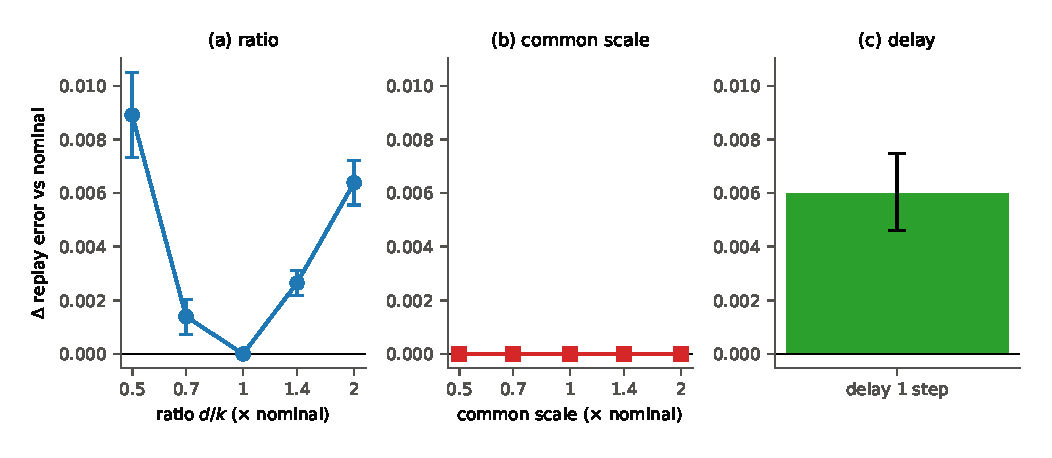
\includegraphics[width=\textwidth]{Fig1}
\caption{Conditional replay-loss responses}\label{fig1}
\figurenote{Mean paired changes from nominal in Eq.~\eqref{eq:loss}, using 98 BridgeData V2 demonstrations on ManiSkill3. Bars: pointwise 95\% paired-bootstrap intervals (10,000 draws). (a) Gain ratio $d/k$, with nominal damping and no delay; (b) common gain scaling, with fixed ratio and no delay; (c) zero versus one-step delay at nominal gains. Horizontal axes in (a,b) are logarithmic; vertical scales are shared. Hollow markers are nominal references, zero by definition; lines guide the eye. These conditional comparisons do not identify a global minimum.}
\end{figure*}

\subsection{Calibration compatibility and the nominal operating point}\label{subsec4_4}

Inverting the calibration test requires a search domain, a loss, a reference and a threshold, and the
answer depends on all four, so we state them. The domain is the 50-point grid of
$(\text{stiffness scale}, \text{damping scale}, \text{execution delay})$ that the replay sweep
enumerates; the loss is the per-demonstration composite objective of Eq.~\eqref{eq:loss}, which sums
a position error in metres and an orientation error in radians; the reference is the
grid's loss minimiser; and a candidate is retained when the one-sided $95\%$ lower bound of its
paired mean loss increase over that minimiser does not exceed zero, which is the rule
Appendix~\ref{secA} states. Computed that way on the 98 common demonstrations,
the loss has a sharply two-part structure.

\paragraph{The loss varies primarily with $(d/k, \text{delay})$.}
Grouping the 50 grid points by ratio and delay gives 26 groups, of which 14 contain two or more
points that differ only in the common scale. These 14 groups span seven distinct ratios from
$0.5$ to $2.0$. Within each group, the mean loss varies by at most $7.2\times10^{-6}$,
with the same bound on both stacks. Between groups it ranges over $6.0\times10^{-2}$, which is $8{,}354$ times the
largest within-group spread on ManiSkill3 and $8{,}767$ times on the original stack. Extending to
the sixteenfold range the policy sweeps actually use ($\times\tfrac14$ to $\times 4$, measured on
the original stack), the largest mean paired loss difference from nominal is $3.1\times10^{-6}$.
All loss figures in this section are in the composite units of Eq.~\eqref{eq:loss}, not in metres.

This is the insensitivity of Sect.~\ref{subsec4_2}(i) measured on the calibration objective itself
rather than on a trajectory. It is verified at seven ratios, without a guarantee at untested ratios. Ratio $0.25$ has exactly
one grid point per delay value, so the common scale is not varied there. This limitation matters in
Sect.~\ref{subsec7_7}, because $0.25$ is the ratio the calibration data prefer.

\paragraph{A zero threshold resolves differences without assessing practical relevance.}
At threshold zero, the rule can reject settings whose loss differences are very small.
Replaying demonstration $m$ at parameter $z$ is deterministic and yields the same loss on every
repetition. The only randomness is which demonstrations were drawn. With 98 paired
demonstrations, the bootstrap resolves mean differences of order $10^{-7}$ in composite loss. At
threshold zero the rule therefore rejects $\times 2$ and $\times 4$ common rescalings whose
mean loss differs from nominal by $4.9\times10^{-7}$ and $7.4\times10^{-7}$, some two to three
thousand times below $\tau$. As the demonstration count grows, the retained
set can shrink towards the loss minimiser. These rejections resolve small differences over sampled
demonstrations; they do not by themselves establish practical relevance.

\paragraph{A reference magnitude for engineering relevance.}
To distinguish statistical detectability from engineering relevance, we additionally evaluate a
nonzero margin. The two stacks implement the same nominal dynamics, and on the same 98 demonstrations
their losses differ by $1.36\times10^{-3}$ in composite units, $95\%$ CI
$[0.61, 2.10]\times10^{-3}$, decomposing into $0.47$~mm of translation and $0.88$~mrad of rotation;
the mean absolute per-demonstration disagreement is $2.76\times10^{-3}$. Two independent
implementations of one set of equations differ by that much, so we use it as a reference magnitude
$\tau = 1.36\times10^{-3}$, reading the set at $\tau$ as well as at zero and reporting
$2.10\times10^{-3}$ as a sensitivity.

This between-stack discrepancy is an engineering reference, not a resolution limit: a same-stack paired
parameter effect can be both smaller than a fixed cross-stack offset and perfectly well resolved,
since the two quantities have different sources of variation. What $\tau$ buys is a scale that was
not chosen to produce an answer. It does not license the claim that anything below it is
unattributable. The signed mean, the mean absolute difference and a quantile are alternative
reference summaries; they differ here by a factor of two, so we report which we used.

\paragraph{Small within-fibre changes and sensitivity of nominal membership.}
Against $\tau$, the iso-scale family ($\le 3.1\times10^{-6}$) is retained by a factor of $440$ and
the halved torque limit ($\le 1.8\times10^{-8}$) by a factor of $75{,}000$. No conclusion in
Sects.~\ref{subsec4_2} and~\ref{subsec4_3} depends on the threshold.

Nominal is the opposite case. The grid's loss minimiser is not the simulator's shipped controller:
on both stacks independently it lies at one step of execution delay and a gain ratio of
$0.25$ to $0.36$, while nominal sits at ratio $1$ with no delay and ranks fifth of 26 groups.
Nominal's paired mean loss increase over the minimiser is $+2.90\times10^{-3}$ with a $95\%$ lower
bound of $+2.25\times10^{-3}$ on ManiSkill3, and $+2.26\times10^{-3}$ with $+1.49\times10^{-3}$ on
the original stack; the ManiSkill3 figure decomposes into $1.06$~mm of translation and $1.84$~mrad
of rotation. Both bounds exceed zero and both exceed $\tau$; at the $2.10\times10^{-3}$ sensitivity
nominal is still out on ManiSkill3 and comes in on the original stack. So its membership is
borderline, and the exact grid point depends on the objective's rotation weight: under
rotation weights from $0$ to $5$ the ManiSkill3 minimiser is unchanged while the
original-stack minimiser moves among three adjacent points. What survives every weight is the
qualitative statement: both stacks prefer one step of delay and a ratio well below $1$, and
neither prefers nominal. The preferred setting therefore depends on the specified objective, whereas the preference
for delay and a lower ratio persists over the tested weights.

\paragraph{Nominal exclusion under sample splitting.}
The rule above selects its reference from the same demonstrations it tests on, which
Sect.~\ref{subsec3_2} shows invalidates the coverage reading, so we assess the exclusion using independent reference selection and testing. Selecting the reference on one half of the
98 demonstrations and testing on the other gives independent selection and inference. Nominal is
still excluded: on ManiSkill3 its paired mean loss increase over the half-sample reference is
$+2.80\times10^{-3}$ composite with a one-sided lower bound of $+1.90\times10^{-3}$, and on the
original stack $+2.49\times10^{-3}$ and $+1.43\times10^{-3}$ respectively. Across five random splits the lower bounds run from
$+1.02\times10^{-3}$ to $+3.03\times10^{-3}$ and nominal is
excluded in all ten stack--split combinations, with the minimiser at delay $1$ and ratio $0.25$ or
$0.35$ every time. Thus the exclusion also holds when reference selection and testing use
independent samples.

Fixing nominal as the test reference would make its own loss increase zero by construction and
prevent the test from rejecting it. This illustrates why the reference must be stated explicitly;
Supplementary Material S1 records the corresponding analysis revision.

The measured insensitivity in Sects.~\ref{subsec4_2} and~\ref{subsec4_3} is independent of that
reference: those sections quantify small within-fibre changes, rather than membership under every
threshold. The set used for the policy verdicts must therefore be distinguished from $C_\alpha$. All
of the main policy sweeps are anchored at nominal; Sect.~\ref{subsec7_7} separately considers the
fitted point. The nominal conditions are the operating point together with
settings with small measured replay changes relative to it: common rescalings
$\times 0.25$ and $\times 4$, the halved torque limit, and contact parameters the free-space replay
never sees at all. That collection is the \emph{calibration-invisible fibre} through the benchmark's
operating point,
\begin{equation}\label{eq:cset2}
\begin{split}
F_{\mathrm{nom}} = {}
  &\{d/k = 1,\ \text{delay}\ 0\}
   \times \{\text{scale} \in [\tfrac14, 4]\} \\[-2pt]
  &\times \{\tau_{\max}/\tau_{\max}^{\mathrm{nom}} \in [\tfrac12, 1]\} \\[-2pt]
  &\times (\text{contact axes, unobserved}),
\end{split}
\end{equation}
where the scale and torque intervals describe the ranges spanned by our tested settings; we do not
claim a continuous-domain guarantee from those finite measurements. The insensitivity argument of
Sect.~\ref{subsec4_2} is a statement about a mechanism, and a mechanism has a domain. A common gain
rescaling leaves the free-space response unchanged to the order the demonstrations excite, which our
measurements confirm over $\times \tfrac14$ to $\times 4$ and which we do not claim beyond it; an
inactive saturation limit is invisible only while it stays inactive, which bounds the torque
statement below rather than at arbitrarily small $\tau_{\max}$. The contact axes are different in
kind: they are unobserved rather than measured flat. They remain unconstrained by this loss within the
admissible parameter domain, reflecting
the protocol's coverage.

$F_{\mathrm{nom}}$ characterises sensitivity around the benchmark's nominal operating point;
$C_\alpha$ characterises compatibility relative to a loss minimiser. The former fixes nominal's
ratio and delay, whereas the latter permits different values on those axes. Keeping these objects
separate makes the scope of each ranking comparison explicit.

The remaining question is whether the ranking at nominal persists at the operating point
preferred by re-calibration. Sect.~\ref{subsec7_7} repeats the complete configuration census on two
tasks at $(k{\times}2,\ d{\times}0.5,\ \text{delay}\ 1)$, with the same configurations, policy seeds
and other evaluation settings.
The point-calibration verdict changes on both eggplant and spoon. The set-valued verdict is
unchanged on eggplant but changes on spoon: a declaration supported by both criteria at nominal
becomes an abstention, with a resolved change of $-0.271$ in the policy gap. Neither criterion
protects against this change of operating point. The two points differ along the gain ratio and
delay, which the calibration data identify; an envelope over either point's invisible fibre
does not cover the move between them.

Together, these analyses distinguish sensitivity within a sampled fibre from sensitivity to
its operating point. The latter is evaluated in Sect.~\ref{subsec7_7}, subject to the demonstration
provenance limits in Sect.~\ref{subsec4_3}.

%%=============================================================================%%
\section{What a finite benchmark measures}\label{sec5}

\subsection{The benchmark is a finite population of configurations}\label{subsec5_1}

Let $e\geq0$ denote the integer episode index, and let $n_{xy}$ and $n_{quat}$ be the numbers of positions and orientations. Both ports map $e$ to position and orientation indices on a fixed grid of initial states,
\begin{align}
\mathrm{pos}  &= \big\lfloor (e \bmod (n_{xy} n_{quat})) / n_{quat} \big\rfloor, \\
\mathrm{quat} &= e \bmod n_{quat},
\end{align}
so the number of distinct initial configurations is $n_{xy} \cdot n_{quat}$, and any episode index
beyond that repeats an earlier initial configuration; policy randomness can still change its
outcome. Object scale is drawn from the asset table, but every
object has a single admissible scale, so it adds no variation.

We abbreviate the four tasks in Table~\ref{tab2} as eggplant, spoon, carrot and cube stacking, respectively.

\begin{table*}[t]
\centering
\begin{lrbox}{\tablecontentbox}
\begin{tabular}{@{}lrr@{}}
\toprule
Task & Original stack & ManiSkill3 port \\
\midrule
Put eggplant in basket & $8 \times 3 = 24$ & $8 \times 8 = 64$ \\
Put spoon on towel & $12 \times 2 = 24$ & $12 \times 2 = 24$ \\
Put carrot on plate & $12 \times 2 = 24$ & $12 \times 2 = 24$ \\
Stack green on yellow cube & $24 \times 1 = 24$ & $24 \times 1 = 24$ \\
\bottomrule
\end{tabular}
\end{lrbox}
\begin{minipage}{\wd\tablecontentbox}
\caption{Initial configuration counts across simulator ports}\label{tab2}
\usebox{\tablecontentbox}
\tablenote{\textit{Notes.} Counts are positions $\times$ orientations. Eggplant also differs in its quaternion values, so matching episode indices do not identify matching scenes across ports.}
\end{minipage}
\end{table*}

Three consequences follow, and all three are visible in published practice.

\begin{enumerate}
\item \textbf{Beyond the grid, initial configurations repeat.} A ``96-episode'' evaluation of the
eggplant task on the ManiSkill3 port is 64 distinct scenes, 32 of which are visited twice.
\item \textbf{The two ports do not evaluate the same benchmark.} For the eggplant task they differ
in the number of orientations (3 versus 8) and in the quaternion values themselves: the best matching
pair has $|\langle q_1, q_2 \rangle| = 0.54$. Per-episode agreement between the ports is therefore
meaningless for that task. Spoon and carrot share their grids exactly, and their cross-port
per-episode agreement is 0.71--0.96, against chance level for eggplant. That contrast is the control
for this diagnosis.
\item \textbf{One scene is worth $1/24$ or $1/64$.} On a 24-configuration task, any reported
difference below 0.042 is less than one scene.
\end{enumerate}

\subsection{The official protocol is already a census}\label{subsec5_2}

The reference protocol repeats a complete enumeration of the 24 initial configurations for each Bridge task under three fixed policy seeds: 72 episodes in total, exactly the denominator of the published table (for instance $31/72 =
0.431$ and $41/72 = 0.569$ for the two Octo variants on the eggplant task). The ManiSkill3 port's
evaluation protocol instead defaults to 100 consecutive episode indices beginning at a configured offset, aligning with
neither the grid nor the seed repetition. The reference protocol therefore already enumerates the configuration population; the port's
default episode schedule differs in its coverage and repetition pattern.

\subsection{What counts as a replicate depends on the policy}\label{subsec5_3}

A policy seed is a replication axis only if the policy consumes it. Octo's diffusion action head
draws a pseudorandom key that enters sampling, so changing the seed produces a new sample and
configuration $\times$ seed is a replication axis. OpenVLA decodes greedily with
sampling disabled, so its policy sampling seed is unused; changing that seed adds no policy-noise
replicate, although execution drift remains possible. Empirically, two ``seed sets'' of this policy are record-identical in 48 of
48 episodes. For such a policy, changing the policy sampling seed supplies no independent replicate; the
configuration grid remains enumerable, while any execution drift requires separate measurement.
Supplementary Material S1 records the correction to the replication claim.

\subsection{Two estimands, two intervals}\label{subsec5_4}

Two different quantities are both legitimate, and they carry different uncertainty.

\emph{(i) The benchmark value} is the number this benchmark reports. After a census, configuration
sampling error is zero and only policy noise and run-to-run numerical noise remain, so
\begin{equation}\label{eq:var}
\mathrm{Var}(\hat\Delta) = N^{-2} \sum_{c} \big[ s^2_A(c)/S_c + s^2_B(c)/R_c \big],
\end{equation}
with $S_c$ and $R_c$ the number of runs of each policy at configuration $c$. ``Run'' means one
episode, and the count is pooled across seed sets: a configuration that received six
episodes contributes $S_c = 6$, even where those episodes came from fewer seed sets. This choice
affects two verdicts: an alternative implementation averages within each seed set at a fixed configuration and takes each seed-set mean
as the observation. Section~\ref{subsec7_2} reports both analyses and explains why we prefer
pooled episode observations.

\emph{(ii) The generalisation value} is performance on comparable scenes. Here configuration
sampling error is real and the appropriate estimator is a paired bootstrap clustered by
configuration.

Equation~\eqref{eq:var} requires variance imputation where replication is insufficient. A configuration with a single run supplies no within-configuration variance, so $s^2(c)$ is
unavailable there. Where the cell has other configurations with two or more runs we substitute the
mean of the measured $s^2$; where no configuration has a replicate we fall back to the
binomial $\bar p(1 - \bar p)$; and for a policy that decodes deterministically, whose re-runs are
record-identical, we set the term to zero and label the cell as carrying no measurement of run-to-run
drift. The 18 rows in the release's core table comprise 15 labelled empirical on both sides,
2 with an empirical term and a deterministic-zero OpenVLA term whose drift is unmeasured, and
1 with a binomial fallback for both policies. Every row prints its
model, so a reader can see which interval rests on an imputation; the imputation is a pooled
variance, which is an assumption of homogeneity across configurations that we do not test and that
would be optimistic if run-to-run noise were concentrated in a few scenes.

Three additional requirements govern variance estimation. With a single run per configuration,
the binomial fallback makes estimator (i) coincide with the ordinary binomial interval:
a census removes configuration sampling error, but estimating policy noise still requires
replication. Independent runs should therefore follow complete grid enumeration.
Record-identical re-runs of a deterministic policy must be merged into one observation;
otherwise, the estimated variance is halved without additional information. Estimator (ii)
must cluster by configuration. This widens intervals by a median factor of 1.04 on the
64-configuration task and up to 1.33 on a 24-configuration task run for 96 episodes.
No verdict changes, but the effective sample size remains necessary for interpreting the intervals.

\subsection{Sensitivity to evaluation protocol and implementation build}\label{subsec5_5}

Holding the configuration grid fixed, we separated three further sources.

\begin{remark}[Scope of the quantities in this paper]\label{rem:scope}
Unless a number is explicitly labelled otherwise, every effect size and interval we report is
census-scope at five seed sets where five exist: the task's configuration grid is fully enumerated,
so configuration sampling error is exactly zero, and the policy-noise term is estimated across as
many independent seed sets as that task has. Five is the count for the eggplant census; the spoon
and carrot sweeps have two, and Appendix~\ref{secC} gives the per-cell figures. Where a quantity is also available at the three-seed budget the reference protocol uses, we
give both and say which is which, because the difference between them is itself one of the paper's
results (Sect.~\ref{subsec7_2}).
\end{remark}

For Table~\ref{tab3}, the seed statistic is the median over policy pairs on episode indices common to all five seed sets. Using a separate intersection for each pair gives $0.068$ instead of $0.067$; the difference is a scope restriction, not rounding. The two builds agree on outcomes for 0.73--0.88 of matched episodes. The four texture variants give $\Delta = +0.213, +0.120, +0.200, +0.053$, whose span is the quantity reported in the table.

\begin{table*}[t]
\caption{Variation remaining after configuration enumeration}\label{tab3}
\begin{tabular}{@{}llll@{}}
\toprule
Source & Isolation & Quantity & Magnitude \\
\midrule
Policy seed & different seeds, same build & sd of $\Delta$ over seed sets & $0.067$ \\
Implementation build & same seeds, newer build & shift in $\Delta$ & $-0.109$ \\
Robot texture variant & texture only; physics fixed & span of $\Delta$ over 4 variants & $0.160$ \\
\bottomrule
\end{tabular}
\tablenote{\textit{Notes.} Entries are distinct statistics of the policy difference $\Delta$, not changes in a single policy's rate, and are not directly rankable. Seed row: five seed sets on the eggplant census. Build row: one run per build on that census. Texture row: one run per configuration on the 300-configuration fractal census. Build and texture rows have no seed replication. Seed and build comparisons use matched episode indices.}
\end{table*}

The third row compares four recolourings of the robot model. These leave all physical properties unchanged,
including masses, friction coefficients and joint limits. The published figure for this task is the mean over all four. On the fractal coke-can census
the four variants give one policy 0.000, 0.280, 0.013 and 0.400, so evaluating on a single variant
displaces the reported number by $-0.173$ to $+0.227$ relative to the four-variant mean. For
comparison, the can's physical orientation, which does change the dynamics, spans only 0.140.

This axis is invisible to replay calibration for the same reason the torque limit is
(Sect.~\ref{subsec4_2}): it never enters the demonstration trajectory. Unlike the torque limit it is
not even a physical parameter, which makes it the paper's sharpest illustration that
``calibration-invisible'' is a property of the protocol's coverage rather than of physics. That a
visual variant should affect a vision-conditioned policy is not itself surprising; it is the
premise of visual domain randomisation \citep{tobin2017domain}.

The suite documents visual matching and variant aggregation as part of its evaluation protocol
\citep{li2024simpler}. We examine the estimand defined by that aggregation. The published success
rate is marginal over a uniform mixture of four variants, whereas evaluation on one variant
estimates a conditional success rate. On this task, the four conditional rates span 0.400.

This distinction has two implications. First, comparing the published rate with a reproduction
on one robot texture compares a marginal and a conditional quantity. The resulting discrepancy
is $-0.173$ to $+0.227$ here even when both computations are correct. Second, complete enumeration
eliminates sampling error from the variant axis because every variant is evaluated. The
0.400 spread is the range of conditional rates, not uncertainty in the published marginal rate;
their deviations from that marginal are $-0.173$ to $+0.227$. Treating the four variants as
replicates of a common quantity and calculating a standard error across them would conflate
these estimands. The measured magnitudes complement the suite's observation that simulated
success rates depend on visual matching.

Whether the axis can flip a ranking rather than widen one policy's interval is a separate
question, and Sect.~\ref{subsec8_4} answers it on a second policy over the same grid. It can move a
verdict to abstention, but it does not reverse an ordering: all twelve texture $\times$ condition
cells there keep the same sign.

The seed and build comparisons use matched episode indices. The pre-fix build and one seed set
contain 96 episodes, whereas the other batches contain 64. Because indices beyond the grid size
repeat configurations, averaging each batch over all its records assigns different effective
weights to configurations and changes the estimated effect by roughly a factor of two.
We report paired results; the companion analysis also provides unpaired results for comparison.
The build-induced shift in $\Delta$ and the policy-seed standard deviation of $\Delta$ describe
different quantities and should not be ranked directly by magnitude.

Two further practical consequences follow. First, a declaration from one seed set need not persist
under replication. The single-seed estimate for Octo-Small minus Octo-Base, $\Delta = +0.250\,[+0.08,
+0.32]$, supported Octo-Small, whereas three seed sets from a single build give $+0.141 /
-0.031 / -0.047$. The single-seed declaration is therefore not retained;
its provenance is documented in Supplementary Material S1. Second, pooling runs across builds inflated the measured seed standard
deviation from 0.055 to 0.093. Runs from different builds must be distinguished when estimating
within-build policy noise. The observed inflation shows contamination by build drift; it does not
provide an additive decomposition of the two variance components.

\begin{figure*}[t]
\centering
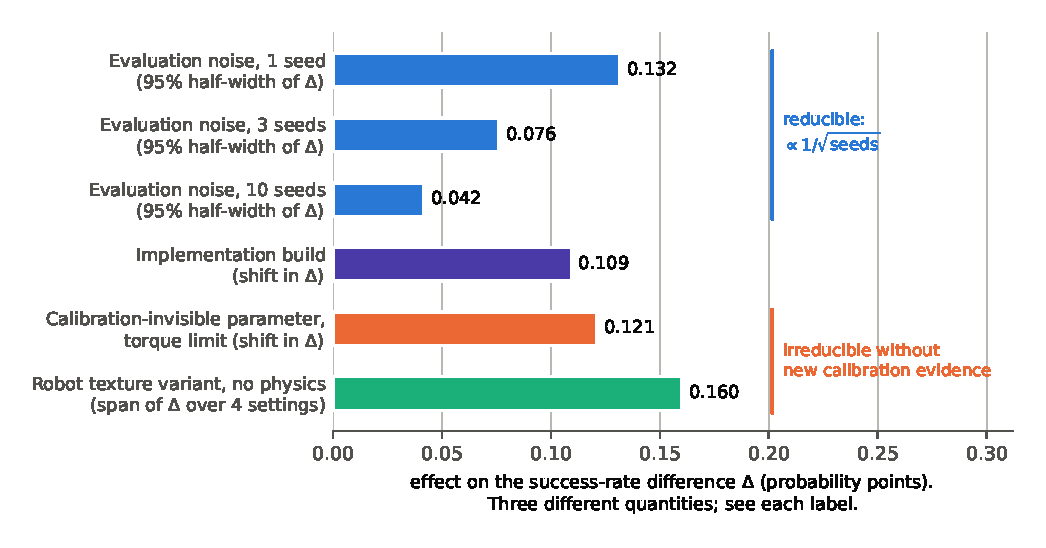
\includegraphics[width=\textwidth]{Fig2}
\caption{Uncertainty after configuration enumeration}\label{fig2}
\figurenote{All bars use policy-difference units $\Delta$, but represent different quantities: 95\% interval half-widths, shifts or spans across four settings, as labelled. Their lengths are not directly rankable. The build bar shows the maximum absolute shift across the two compared conditions. Evaluation-noise terms decrease as $1/\sqrt{S}$; the build, torque-limit and texture terms do not decrease with repeated evaluation. Seed, build and texture scopes are given in Table~\ref{tab3}; the torque-limit comparison is described in Sect.~\ref{subsec7_3}.}
\end{figure*}

\subsection{Reporting requirements}\label{subsec5_6}

For each reported estimate, we specify the number of configurations covered and the total number
of configurations; the number of runs per configuration and whether they are independent for that
policy; the variance model (empirical, binomial fallback, or unmeasured); the target estimand; and
the simulator port and implementation build used. Build provenance is recorded separately for each run in an append-only log. Metadata overwritten by later runs cannot establish the provenance of earlier episodes.

%%=============================================================================%%
\section{Reproducing the published protocol}\label{sec6}

\subsection{Reference protocol and RNG lifecycle}\label{subsec6_1}

For each Bridge task, the reference protocol comprises three runs with different fixed policy seeds.
Each run enumerates all 24 initial configurations, yielding 72 episodes in total, the denominator
of the published rates.

The policy's pseudorandom state is initialized once at the start of each run and advances
throughout that run, including across episode boundaries. Episode resets restore the task,
observation history and action-processing state without reseeding. Each seed therefore
initializes a complete run, rather than a separate episode.
For comparison, we also report a per-episode-re-seeding variant in which all 24 configurations
within a run start from the same policy random state. This variant arose from a reproduction error
documented in Supplementary Material S1; it changes agreement with the published table, the across-run
spread and the sign of one comparison (Sect.~\ref{subsec6_3}). All numbers below use the reference
lifecycle unless labelled otherwise.

We reproduced this on the original reference stack, running headless through the Vulkan compatibility
layer of Appendix~\ref{secB}, with the policies served by our own inference server rather than
in-process. Published values are read from the pinned metrics table distributed with the benchmark.
For the reference-protocol runs, each episode reset verifies that the policy random state is initialized for the first episode and retained thereafter.
The companion analysis reports the reference and per-episode-re-seeding lifecycles side by side.

\subsection{Reproduction discrepancies and their direction}\label{subsec6_2}

\begin{table*}[t]
\caption{Reproduced and published success rates}\label{tab4}
\begin{tabular}{@{}llrrrrrrr@{}}
\toprule
 & & \multicolumn{4}{c}{reference lifecycle} & & & re-seeding \\
\cmidrule(lr){3-6}
Task & Policy & seed 0 & seed 2 & seed 4 & pooled & published & diff. & pooled \\
\midrule
Eggplant & Octo-Small & 0.542 & 0.500 & 0.542 & 0.528 & 0.569 & $-0.041$ & 0.556 \\
Eggplant & Octo-Base & 0.458 & 0.417 & 0.417 & 0.431 & 0.431 & $-0.000$ & 0.472 \\
Spoon & Octo-Small & 0.375 & 0.417 & 0.333 & 0.375 & 0.472 & $-0.097$ & 0.431 \\
Spoon & Octo-Base & 0.042 & 0.000 & 0.000 & 0.014 & 0.125 & $-0.111$ & 0.083 \\
Carrot & Octo-Small & 0.042 & 0.042 & 0.167 & 0.083 & 0.097 & $-0.014$ & 0.069 \\
Carrot & Octo-Base & 0.042 & 0.083 & 0.042 & 0.056 & 0.083 & $-0.027$ & 0.125 \\
Cube stacking & Octo-Small & 0.000 & 0.042 & 0.042 & 0.028 & 0.042 & $-0.014$ & 0.042 \\
Cube stacking & Octo-Base & 0.000 & 0.000 & 0.000 & 0.000 & 0.000 & $+0.000$ & 0.000 \\
\bottomrule
\end{tabular}
\tablenote{\textit{Notes.} The reproduction uses 72 episodes per task and policy under the reference RNG lifecycle; the last column uses earlier per-episode re-seeding. The eight cells share tasks, policies and seeds and are not independent replications. For eggplant, Octo-Base's $0.4306$ rounds to the published $0.431$; its displayed negative zero is a rounding effect.}
\end{table*}

Table~\ref{tab4} reveals both moderate discrepancies and a common direction.

The magnitudes are small. The policy-seed noise we measure on the 64-configuration eggplant census is
$\pm 0.132$ at half-width for a single seed set and $\pm 0.076$ for three.
Every cell's discrepancy is below the single-seed reference
half-width, although these eggplant figures are not uncertainty bounds for the other tasks. Those two
figures come from the spread of $\hat\Delta$ across whole seed sets. The median
$\mathrm{sd} = 0.068$ over pairs and conditions is scaled as $1.96\,\mathrm{sd}/\sqrt{S}$.
This noise model differs from Eq.~\eqref{eq:var}, the estimator every table in this paper uses. Eq.~\eqref{eq:var}
pools per-configuration run variances and gives per-pair three-seed half-widths of $0.075$--$0.088$
on the same census (Sect.~\ref{subsec7_6}). The two answer different questions: how far a
whole-census result moves between seed sets, and how precisely one census estimates the benchmark
value. We report them separately rather than treating them as one quantity. The reproduction
uses a different operating system, a software-rendered rasteriser, a different graphics path and an
out-of-process policy server. This check quantifies the resulting agreement with published rates;
it does not isolate those components or establish their equivalence. On the second embodiment the same check gives $+0.003$
(Octo-Base on Coke-can grasping, 0.173 against 0.170 published) and $-0.040$ (RT-1-X, 0.527 against
0.567).

The discrepancies have a common direction: six of the eight cells fall below the published
value, two match it, and none exceeds it; the mean difference is $-0.038$.
This pattern is descriptive and does not identify a platform-wide correction.

The eight cells are four tasks crossed with two policies sharing seeds, rather than eight
independent measurements of one platform. A $t$ interval that treated them as independent would
not justify a platform-wide inference. The published rates are also point estimates without
intervals, so their evaluation noise can contribute to the discrepancies. The lifecycle comparison
is descriptive rather than causal: the per-episode-re-seeding variant has a mean difference of
$-0.005$, a mean absolute discrepancy of $0.026$, and a mean across-run range of $0.109$, compared with $0.052$ under the reference
lifecycle. Three runs per cell are insufficient to establish that extra variance concealed a
systematic gap. The non-reference variant agrees more closely with the published rates, while the
reference lifecycle has a larger discrepancy in a common direction; closer numerical agreement
alone therefore does not establish protocol fidelity.

The mean absolute difference $0.038$ is about a third of the $0.121$ torque shift,
and the largest cell difference, $0.111$, is comparable to that shift. Relative to the
$0.400$ texture range, the mean discrepancy is about ten times smaller. These comparisons
do not establish that pipeline differences are negligible. The main analyses in
Sects.~\ref{sec5}--\ref{sec8} compare two policies on the same configuration, pipeline and build.
An offset common to both policies cancels in their difference; a policy-specific interaction
does not. In particular, the build change in Sect.~\ref{subsec5_5} moves $\hat\Delta$ by
$-0.109$ and therefore cannot be treated as a common offset. The mean difference of $-0.038$
must remain explicit when comparing our absolute rates with the published rates in this section.

\subsection{What the published budget resolves}\label{subsec6_3}

The same table answers a second question, and the answer is less comfortable. Even under the
reference lifecycle the three runs disagree with each other by more than we differ from the published
value: the across-run range of a cell averages 0.052 and reaches 0.125. Applying the census estimator
of Sect.~\ref{subsec5_4} to the comparison the published protocol is built to support gives
Table~\ref{tab5}.

\begin{table*}[t]
\caption{Policy orderings at the published evaluation budget}\label{tab5}
\begin{tabular}{@{}lrllrrl@{}}
\toprule
 & \multicolumn{3}{c}{reference lifecycle} & & \multicolumn{2}{c}{re-seeding} \\
\cmidrule(lr){2-4}\cmidrule(l){6-7}
Task & our $\Delta$ & census 95\% & verdict at this budget & published $\Delta$ & $\Delta$ & verdict \\
\midrule
Eggplant & $+0.097$ & $[-0.042, +0.236]$ & abstain & $+0.138$ & $+0.083$ & abstain \\
Spoon & $+0.361$ & $[+0.259, +0.463]$ & S $\succ$ B & $+0.347$ & $+0.347$ & S $\succ$ B \\
Carrot & $+0.028$ & $[-0.039, +0.094]$ & abstain & $+0.014$ & $-0.056$ & abstain \\
Cube stacking & $+0.028$ & $[-0.011, +0.066]$ & abstain & $+0.042$ & $+0.042$ & abstain \\
\bottomrule
\end{tabular}
\tablenote{\textit{Notes.} Reference-lifecycle intervals use Eq.~\eqref{eq:var}: policy noise only, with $S=3$ runs over all 24 configurations. The final two columns show the per-episode-re-seeding comparison. S and B denote Octo-Small and Octo-Base, respectively.}
\end{table*}

Four observations.

\paragraph{(i) One of four orderings is resolvable.}
Only the spoon comparison excludes zero. On the other three tasks our reproduction at the published
budget does not resolve the ordering under the stated variance model. The published tables report
rates rather than rankings. For readers comparing these rates across policies, our results show
why point differences alone do not establish an ordering; they do not identify an error in the
reference implementation.

\paragraph{(ii) The unresolved carrot comparison is sensitive to the RNG lifecycle.}
On carrot, the per-episode-re-seeding variant gives $-0.056$ for Octo-Small minus Octo-Base,
opposite to the published $+0.014$. Under the reference RNG lifecycle the difference is $+0.028$,
with interval $[-0.039, +0.094]$, and no cell in Table~\ref{tab5} disagrees in mean sign with the
published table. The re-seeding variant starts all 24 configurations in a run from the same policy
random state and does not reproduce the reference sampling protocol.
The data therefore support an unresolved ordering at this budget, not a reversed ordering under
a faithful reproduction. Supplementary Material S1 records the earlier interpretation and its correction.

\paragraph{(iii) Removing configuration sampling error is not enough.}
The census interval is narrower than the binomial-over-72 a reader of the published table would
compute on three of the four tasks and marginally wider on the fourth: half-widths 0.139 against
0.163 on eggplant, 0.102 against 0.115 on spoon, 0.067 against 0.083 on carrot, and 0.039 against
0.038 on cube stacking. No verdict changes either way. With three runs per configuration the
per-configuration policy variance dominates, so enumerating the configuration grid, which sets the
sampling error to exactly zero, does not eliminate the remaining uncertainty. Once the grid is
covered, additional budget should provide independent policy runs rather than count repeated initial
configurations as new scenes.

\paragraph{(iv) Sensitivity to the variance model.}
``One of four'' is not model-free. Eq.~\eqref{eq:var} treats each configuration's runs as the
replication unit and pools the per-configuration policy variances; on the new records that gives the
intervals in Table~\ref{tab5} and one resolvable ordering. An alternative treats each of the
three runs as the unit and constructs a paired $t$ interval on three whole-census block differences. This gives
eggplant $[+0.038, +0.157]$, spoon $[+0.242, +0.481]$, carrot $[-0.188, +0.243]$, cube stacking
$[-0.032, +0.088]$, hence two resolvable orderings. The block interval is not automatically
better: with three blocks it rests on two degrees of freedom, and eggplant's three block differences
happen to fall close together, which is what makes that interval narrow.

We report Eq.~\eqref{eq:var} as the headline under the assumption that advancing-stream draws
provide independent episode-level policy noise, with no additional shared run effect. Under the
reference lifecycle each episode uses a different segment of the advancing stream, whereas our
earlier re-seeding lifecycle deliberately reused the same initial random state. Stream advancement
alone does not establish independence or rule out shared run effects; the block analysis is therefore
a relevant sensitivity check. The number of resolved orderings is therefore conditional on the
variance model: one of four under the per-configuration estimator and two of four under the
whole-census block analysis.

\subsection{Scope of the reproduction results}\label{subsec6_4}

The three-seed 64-configuration eggplant census has policy-noise half-widths of roughly $\pm 0.08$;
the reference protocol's 24-configuration task-specific intervals are reported separately in
Table~\ref{tab5}. The former magnitude is of the same order as the mean parameter-induced shift of
0.121 associated with the calibration-invisible torque limit in Sect.~\ref{sec7}. These are distinct
quantities, an uncertainty half-width and an observed shift, that need to be reported together.
Section~\ref{subsec6_2} measures agreement with the published implementation, but does not transfer
the port's uncertainty estimate to every published rate.

Two qualifications apply to these reproduction results. Our rates average $0.038$ below the published
ones, so a comparison of absolute rates must disclose that observed discrepancy rather than treat it
as a known correction; the main within-pipeline comparisons in Sects.~\ref{sec7} and~\ref{sec8} are differences between two
policies measured in the same configuration and on one build, where an offset common to both
policies cancels. A build change need not be a common offset (Sect.~\ref{subsec5_5}). The RNG lifecycle is
also part of the protocol: it changed our agreement with the
published table, halved the across-run spread, and decided the sign of one comparison. A reproduction
that matches an outer loop while differing in how policy randomness is threaded through it does
not reproduce the same sampling protocol. Whether that also changes the expected-value estimand
depends on how the random draws enter the policy; the observed changes here already establish the
need to document the lifecycle.

%%=============================================================================%%
\section{Decision-relevant non-identifiability}\label{sec7}

Sections \ref{sec4} and \ref{sec5} showed that the calibration protocol cannot see certain parameter
directions and that the benchmark's own budget leaves its rankings unresolved. Their decision relevance depends on whether moving a parameter along the evaluated invisible fibre
changes a policy comparison. This section measures that effect and tests whether the resulting
verdict changes persist as the evaluation budget increases.

\subsection{Strong and weak forms}\label{subsec7_1}

Fix a task, a policy pair $(i,j)$ and the invisible fibre $F_{\mathrm{nom}}$ of Sect.~\ref{subsec4_4}. The
claim under test is that point calibration and the union envelope disagree: point calibration
declares orderings the calibration data cannot support. Two forms are worth separating.

The \textbf{strong form}: some $z \in F_{\mathrm{nom}}$ reverses a ranking's sign, so that the simulator's
answer to which policy is better depends on a parameter the calibration data are silent about.
We did not observe this form. Across every pair, task and condition we measured, no
calibration-invisible parameter reverses a sign-determined ranking. The negative density-cell estimate observed at a smaller budget also changes sign at five seed sets
(Sect.~\ref{subsec7_5}).

The \textbf{weak form}: the parameter moves $\Delta$ far enough to cross the decision boundary,
turning a declared ordering into an abstention. This occurs in the measured comparisons and depends on the evaluation budget.

\subsection{One pair, end to end}\label{subsec7_1b}

Table~\ref{tab6a} traces one policy pair from calibration sensitivity to the ranking verdict.
This separates that comparison from the largest parameter effect, the surviving point-versus-set
disagreement, and the published real-robot comparison, which involve different pairs or embodiments.
The table note states the remaining cross-stack provenance boundary.

The replay-loss column in Table~\ref{tab6a} describes calibration sensitivity in the composite units of Eq.~\eqref{eq:loss}; $\hat\Delta$ describes the policy difference in probability points. These quantities have different units. An \emph{unobserved} parameter never enters the free-space replay trajectory, so the missing replay measurement reflects a gap in protocol coverage rather than insufficient precision.

\begin{table*}[t]
\caption{Calibration sensitivity and policy verdicts on eggplant}\label{tab6a}
\small
\begin{tabular}{@{}lllrll@{}}
\toprule
Condition & Calib.\ sees it? & Replay-loss change & $\hat\Delta$ & 95\% interval & Verdict \\
\midrule
Nominal & base point & $0$ by construction & $+0.055$ & $[-0.008, +0.117]$ & abstain \\
Gain scale $\times0.25$ & measured flat & $\le 3.1\times10^{-6}$ & $+0.092$ & $[+0.025, +0.159]$ & S $\succ$ B \\
Gain scale $\times4$ & measured flat & $\le 3.1\times10^{-6}$ & $+0.174$ & $[+0.105, +0.244]$ & S $\succ$ B \\
Torque limit $\times0.5$ & measured flat & $\le 1.8\times10^{-8}$ & $+0.106$ & $[+0.040, +0.172]$ & S $\succ$ B \\
Friction $\times0.4$ & unobserved & not in a replay & $+0.077$ & $[+0.015, +0.139]$ & S $\succ$ B \\
Density $\times0.5$ & unobserved & not in a replay & $+0.128$ & $[+0.059, +0.197]$ & S $\succ$ B \\
\midrule
union over the fibre & --- & --- & --- & $[-0.008, +0.244]$ & abstain \\
\bottomrule
\end{tabular}
\tablenote{\textit{Notes.} Multipliers are relative to nominal. Gain scale multiplies arm-joint stiffness and damping equally. Policy comparison: Octo-Small (S) minus Octo-Base (B); all 64 configurations; five seed sets; one inference build; run observations; empirical variances on both sides in Eq.~\eqref{eq:var}. Configuration sampling error is zero. Replay bounds come from ManiSkill2; policy estimates and intervals come from ManiSkill3. These are not matched single-stack measurements. In particular, the sixteenfold gain-scaling replay bound has not been established for an unmeasured ManiSkill3 sweep over the same range (Sect.~\ref{subsec4_4}).}
\end{table*}

Across the fibre, $\hat\Delta$ spans
$0.120$, from $+0.055$ to $+0.174$, and the verdict changes from abstention to declaration.
These conditions have replay-loss differences from nominal of at most $3.1\times10^{-6}$ in composite units,
or no replay measurement because the parameter never appears in the trajectory. The calibration protocol's resolution and the policy
comparison's sensitivity are unrelated in magnitude on this pair, which illustrates the mismatch between calibration resolution and decision sensitivity within
the stated scope.

Table~\ref{tab10} reports the separate operating-point comparison for the same pair, using
three seed sets at each operating point to match the evaluation budget. The $0.121$ torque
shift in Sect.~\ref{subsec7_3} concerns cross-family Octo-versus-OpenVLA pairs; for the
Octo-versus-Octo pair in this table, the same parameter changes $\hat\Delta$ by $+0.051$.
These effect sizes therefore refer to different policy comparisons.

\subsection{Policy comparisons across evaluation budgets}\label{subsec7_2}

The complete per-pair table reports both verdicts for every policy pair on every task, with the
configurations covered, the runs per policy and the variance model for each. It is
available through the companion evidence index (Appendix~\ref{secD}). It has 18
rows: 17 bridge policy pairs across the two ports, plus the Coke-can grasping pair of
Sect.~\ref{subsec8_4}, which we count separately because it is a different embodiment and a
different question. Wherever this paper says ``of 17 pairs'' it means the 17 bridge rows.
Table~\ref{tab6} below is not that table; it shows only the three pairs whose point-versus-set
verdict differs at the reference protocol's three seed sets, and what raising the budget to five
does to each.

The observation unit matters because two defensible choices give different verdicts on two rows. Eq.~\eqref{eq:var} writes $S_c$ for the number of \emph{runs} at
configuration $c$, and that is what we report: episode outcomes pooled across seed sets,
so a configuration that received six episodes contributes six observations. An alternative analysis averages the episodes within each seed set at a configuration and treats each
\emph{seed-set mean} as the observation, making $S_c$ the number of seed sets. The two differ
because seed set B carries 96 episodes on a 64-configuration grid, so episode indices 64--95 wrap onto
configurations 0--31 and give those configurations two episodes with different policy seeds.
In these census records, each episode's policy seed is the sum of its seed-set base value and its episode index. Neither unit is wrong: the run unit is
finer and is what the formula states; the seed-set unit is conservative against a common effect within a seed set, which the build-drift result of Sect.~\ref{subsec5_5} shows can exist across
generations, though the five sets here share one build. We use runs as the primary observation unit to match Eq.~\eqref{eq:var}, and report
seed-set means as a sensitivity analysis. Both analyses are reproducible from the released records. The two units move two
of the eighteen rows: Octo-Small versus Octo-Base on eggplant declares under the
seed-set unit on a lower bound of $+0.000042$ and abstains under the run unit at
$[-0.008, +0.117]$, and Octo-Small versus Octo-Base on the original-stack spoon does
the opposite. The point-versus-set disagreement count is 1 of 17 under both.

For Octo, a single-frame-history variant uses one observation frame; an unqualified model name denotes its default observation history.
Of the 17 bridge pairs, one disagrees: Octo-Base versus Octo-Base (single-frame history) on the
eggplant census, point $\Delta = +0.073\,[+0.01, +0.14]$ declaring Octo-Base better, union
interval $[-0.06, +0.14]$ abstaining.

The union runs over the nominal setting as well as the five calibration-invisible ones, and the
reason is definitional rather than statistical. The set being unioned over is $F_{\mathrm{nom}}$,
the fibre of settings the replay loss cannot distinguish from nominal (Sect.~\ref{subsec4_4}), and
nominal is its base point, so it belongs to the fibre by construction. An envelope taken over the
perturbed conditions alone would not cover the fibre it claims to bound. It widens no verdict in
Table~\ref{tab6}. We note that nominal's membership in $F_{\mathrm{nom}}$ is a tautology and carries
no implication that nominal is the calibration optimum; Sect.~\ref{subsec4_4} shows it is not.

One consequence should be stated plainly, because a reader scanning the table's two-decimal columns
cannot see it. Two declarations rest on a bound that rounds to $+0.01$: Octo-Small versus
Octo-Small (single-frame history) at $+0.0091$, and the surviving disagreement's own point calibration at
$+0.0095$. Put a lower bound of $+0.0095$ in units of the evidence behind it. On a 64-configuration
census with a balanced design of five runs per policy per configuration, $\hat\Delta$ would weight each configuration mean by $1/64$ and each
individual episode by $1/(64 \times 5) = 0.0031$, so $+0.0095$ is about $0.6$ of one
configuration's mean outcome, or about three single-policy episodes out of the 320 on each
side of that balanced comparison. The actual per-configuration counts are unequal
(Appendix~\ref{secC}); this illustration indicates scale rather than the exact influence of each
retained episode. Changing episode outcomes also changes the estimated variance.
Both are formal declarations with small margins, which we flag explicitly rather than obscure
through rounding. The criterion's substantive declarations are the ones with margin,
and the multiplicity analysis below says which those are: the five cross-family Octo-versus-OpenVLA
envelopes that survive a family-wise correction, plus the fractal pair of Sect.~\ref{subsec8_4}. The
spoon envelopes are not among them: $[+0.04, +0.56]$ looks wide but its lower bound is
$+0.035$, and the envelope's binding constraint is that bound rather than the width of the interval,
so it does not survive. That is worth noticing: a wide envelope that only just clears zero is a weak
declaration, not a strong one, and reading the interval's width for its margin gets it backwards. These small-margin declarations are also sensitive to the observation unit.
The largest of them under the seed-set unit was $+0.000042$, on a pair that abstains under the run
unit. A bound that small is a property of the estimator's last digit, not of the policies.

At three seed sets, three rows disagreed. The two that no longer do were resolved by spending seeds,
not by any change of method or of data-retention rule.

\paragraph{Sensitivity to multiple-comparison control.}
Seventeen pairs are seventeen hypotheses, and a reader who scans the table for whichever orderings
it declares is making a family-wise claim. We therefore apply Holm's step-down procedure at
$\alpha = 0.05$ to each rule's 17 $p$ values. Holm needs no independence assumption, and these
pairs are certainly not independent, six of them being drawn from four Octo variants on shared
policy data.

For the envelope, let $p_+(z)$ and $p_-(z)$ be the one-sided normal-model $p$ values for
positive and negative differences at setting $z$. We first form the two directional
intersection--union tests and then allow either ordering:
\begin{align}
 p_+^* &= \max_{z\in S}p_+(z),\qquad p_-^* = \max_{z\in S}p_-(z), \notag\\
 p_{\mathrm{env}} &= \min\{1,\,2\min(p_+^*,p_-^*)\}. \label{eq:directional_iut}
\end{align}
For same-sign estimates this equals the largest two-sided component $p$ value. Mixed-sign
estimates give $p_{\mathrm{env}}=1$ before adjustment across policy pairs. Supplementary
Material S1 documents the implementation correction; the reported declaration counts are unchanged.

\begin{table}[h]
\caption{Policy declarations under different error controls}\label{tab6b}
\begin{tabular}{@{}lrrr@{}}
\toprule
Standard over the 17 pairs & point & envelope & disagree \\
\midrule
no correction across pairs & 11 & 10 & 1 \\
Holm at $\alpha = 0.05$ & 9 & 5 & 4 \\
Benjamini--Hochberg & 11 & 10 & 1 \\
\bottomrule
\end{tabular}
\tablenote{\textit{Notes.} Counts use the same 17 Bridge policy pairs. Point and envelope columns count declarations; the final column counts pairs with different verdicts under the two rules.}
\end{table}

\noindent Point
calibration's 11 declarations fall to 9. The two removed declarations are exactly the marginal cases of the
previous paragraph, at $+0.0091$ and $+0.0095$. The envelope's 10 fall to 5, so the
disagreement between the rules rises from 1 of 17 to 4 of 17. Considering both rules together, correcting for multiplicity makes the set-valued rule more
consequential relative to point calibration, not less, because it removes more of the envelope's
declarations and so turns agreements into disagreements. The four pairs are
Octo-Small versus Octo-Base (single-frame history) and Octo-Base (single-frame history) versus OpenVLA on
the eggplant census, and Octo-Small versus Octo-Base on spoon on each stack.

Three limits on that reading, and we hold to all three. Four extra abstentions are not four
corrected errors. We have no true ordering for these pairs, so we cannot tell an avoided false
declaration from a surrendered correct one, and the two rules are not even answering the same
question: one asks about a single setting, the other about agreement across a set. What is
established is that a declaration is sensitive to the parameter set and to the error-control
standard; that a set-valued rule decides better is not established here and we do not claim
it. Holm needs valid input $p$ values, which ours are only under the normal approximation
and the variance imputation of Sect.~\ref{subsec5_4}; a correction does not repair a calibration
problem in the thing it corrects, so this is a sensitivity analysis under a stated working model
rather than a guarantee. And the direction of the envelope's larger loss is a fact about
these records, not a theorem: an intersection--union test's $p$ value is the largest of its
one-sided components for a fixed direction, followed here by the two-direction correction in
Eq.~\eqref{eq:directional_iut}. Requiring every condition to support the same ordering explains
why the envelope declares less often to begin with, but it does not
determine how a step-down procedure over a different index (pairs, not conditions) will treat
it. None of this touches the no-correction-across-conditions argument of Sect.~\ref{subsec3_3}, and
a correction cannot affect an abstention, since it only removes declarations. Benjamini--Hochberg
leaves every count unchanged; we report Holm because the reading at issue is family-wise rather than
one about a false-discovery rate.

\begin{table*}[t]
\caption{Seed-budget sensitivity of ranking disagreements}\label{tab6}
\begin{tabular}{@{}llll@{}}
\toprule
Pair & Union at $S=3$ & at $S=5$ & Outcome \\
\midrule
S versus B1 & $[-0.020, +0.275]$ abstain & $[+0.012, +0.245]$ declare & withdrawn \\
B1 versus V & $[-0.000006, +0.416]$ abstain & $[+0.017, +0.426]$ declare & withdrawn \\
B versus B1 & $[-0.099, +0.167]$ abstain & $[-0.064, +0.137]$ abstain & survives \\
\bottomrule
\end{tabular}
\tablenote{\textit{Notes.} S and B denote Octo-Small and Octo-Base with default observation history; B1 denotes Octo-Base with single-frame history, and V denotes OpenVLA. Eggplant configuration census; both budgets use the run observation unit. $S=3$ comprises seed sets A$'$, B and C. Envelopes include the nominal setting. The second row's $S=3$ lower bound is $-6\times10^{-6}$, so that abstention is numerically marginal.}
\end{table*}

This budget-sensitivity check reduces the number of point--set disagreements from three to one.
The earlier draft records the intended check, but the available provenance does not independently
establish that it was fixed before the additional evaluations. We therefore treat it as an
exploratory sensitivity analysis (Supplementary Material S1).

The comparison therefore depends on the evaluation budget. At the reference protocol's
three seed sets, point calibration declares orderings the union envelope does not support on
3 of the 17 bridge policy pairs, although one of the three, as the table note states, abstains
by six millionths. At five seed sets over a complete configuration census, one remains. A single
seed set can evaluate only 13 of the 17 pairs at all, and disagrees on 2 of those 13. The
criterion's value is concentrated in the budget
regime practitioners are actually in. This is weaker than the claim we set out to make, and it
remains useful: we are aware of no published evaluation that runs five seed sets over a full
configuration census, and the reference protocol itself uses three. Every count here is reproducible
by restricting the analysis to the specified seed sets.

The remaining disagreement arises from the declaration margin and interval width.
No between-condition sign reversal is resolved (Sect.~\ref{subsec7_5}). The nominal lower bound
is $+0.0095$, whereas the union envelope uses the smallest lower bound across conditions:
$-0.064$ under friction $\times 0.4$. Thus the rules differ between a marginal point declaration
and abstention, without supporting opposite policy orderings.

\subsection{The mechanism: one parameter, measured on a complete census}\label{subsec7_3}

The torque limit is the cleanest case. The replay trajectories are
bitwise unchanged on 97 of the 98 demonstrations and differ by at most 0.050~mm on the remaining
one, consistent with inactive torque saturation over most of the replay set
(Sect.~\ref{subsec4_2}(ii)). Commanded torques were not logged, so the mechanism remains an
interpretation of the trajectory evidence (Sect.~\ref{subsec4_3}). Halving it therefore stays inside
$F_{\mathrm{nom}}$ with a margin set by the mechanism rather than by a fitting tolerance. On the 64-configuration eggplant census it
moves the cross-family comparison by $-0.104$, $-0.146$, $-0.108$ and $-0.127$ for the four
Octo-versus-OpenVLA pairs: a shift of 0.104--0.146, mean 0.121, uniform enough across pairs
to be consistent with a single policy moving rather than four independent effects.

\begin{remark}
The estimated shift depends on configuration coverage and seed budget. On 48 of the 64
configurations it was 0.23--0.25, with two pairs crossing the decision
boundary: the partial census gave a larger estimate. On the complete census at three seed sets it read
0.133--0.161, mean 0.141; at five it has the values reported above. The eggplant torque-shift estimates reported here therefore use the complete configuration
census at $S = 5$, the largest budget examined in Sect.~\ref{subsec7_2}.
\end{remark}

\subsection{Checks on the torque-limit mechanism}\label{subsec7_4}

We assess policy specificity, configuration coverage and task dependence.

\paragraph{It is a property of one policy, and a large one.}
Halving the torque limit raises OpenVLA's eggplant benchmark value from 0.156 to 0.271 on the
complete 64-configuration census ($+0.115$), while Octo-Small, run as a negative control over the
same census, moves by $+0.011$ and the other three Octo policies by $-0.031$ to $+0.006$ with no
consistent direction. The asymmetry is consistent with a contact-torque mechanism: OpenVLA emits larger single-step displacements,
so at the nominal limit it pushes the eggplant away or re-grasps repeatedly on contact, and the
episode-level counters agree (grasp rate $+0.12$/$+0.18$, fewer repeated gripper closures).

\paragraph{It is broad, not driven by a few configurations.}
The configuration-level counts use the same current five-Octo-seed-set scope and estimator as
Fig.~\ref{fig3}, with record-identical whole runs of the deterministic policy deduplicated. Over the complete census 16 configurations improve, 42 are unchanged and 6 degrade, and the mean
change is positive in 7 of the 8 eggplant orientations ($-0.06$ to $+0.29$). The gain is
anticorrelated with nominal success ($r = -0.45$): of the 51 configurations where OpenVLA fails
outright at the nominal limit, 13 are rescued. The parameter repairs failures rather than padding
successes. The same decomposition for Octo-Small has mixed directions: 20 improve, 16
degrade, and 3 of 8 orientations are positive. This is consistent with lower sensitivity to the torque limit.

\paragraph{It is task-dependent in the direction the mechanism predicts.}
On the spoon task (24-configuration complete census) the same parameter produces a small change in $\Delta$
($-0.01$ to $-0.07$ across the four cross-family pairs, against the earlier three-Octo-seed-set
eggplant mean of $-0.14$) and changes no verdict. This is a historical, unmatched-budget
comparison; the current five-seed eggplant estimates are reported in Sect.~\ref{subsec7_3}. This task dependence is consistent with the proposed contact-torque mechanism. A calibration-invisible parameter is therefore not uniformly dangerous: its
decision-relevance is a property of the task-policy pair, which is precisely why it cannot be argued
away a priori and has to be enumerated.

\begin{figure*}[t]
\centering
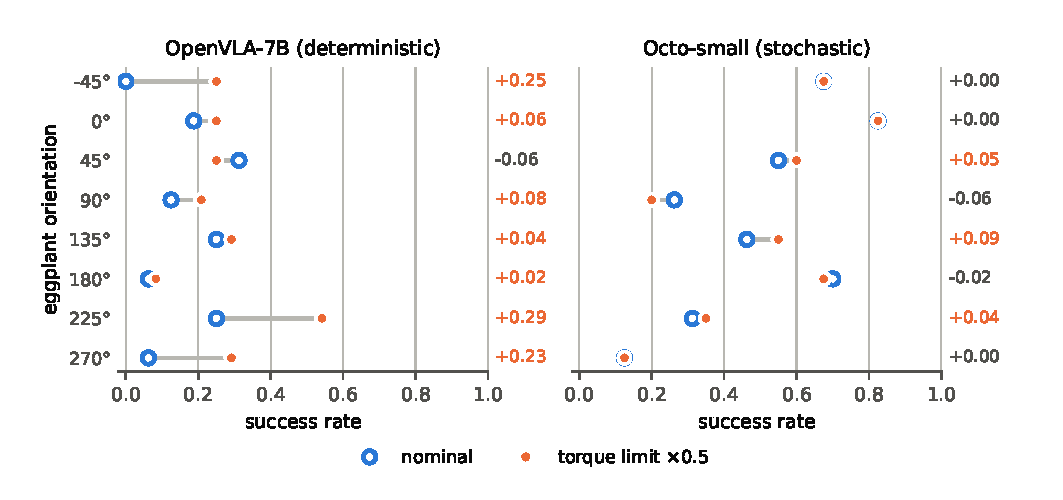
\includegraphics[width=\textwidth]{Fig3}
\caption{Torque-limit effects across eggplant orientations}\label{fig3}
\figurenote{OpenVLA (left) uses deterministic decoding; Octo-Small (right) is stochastic. Estimates and the configuration-level counts in the text use the same current inputs and estimator: five Octo seed sets, with record-identical whole deterministic runs deduplicated.}
\end{figure*}

\subsection{No resolved between-condition sign reversal at five seed sets}\label{subsec7_5}

At a smaller budget, Octo-Base versus Octo-Base (single-frame history) had an estimated
policy difference of $\Delta = -0.021$ under density $\times 0.5$, against positive values under
the other five conditions. At five seed sets the same cell reads
$+0.042\,[-0.024, +0.108]$, and no condition has a point estimate below $-0.001$:
nominal $+0.073$, force $\times 0.5$ $+0.050$, iso $\times 0.25$ $+0.030$, iso $\times 4.0$
$+0.006$, friction $\times 0.4$ $-0.00052$, density $\times 0.5$ $+0.042$. Thus the negative
density-cell estimate does not persist at the larger budget, and the remaining near-zero estimates
do not establish an irreducible parameter-induced reversal. Supplementary Material S1 records
the earlier interpretation and the budget change that resolved it.

This distinction separates parameter sensitivity from evaluation uncertainty. As the evaluation
half-width $h \to 0$ the union envelope converges to
$\big[\min_c \Delta_c, \max_c \Delta_c\big]$, which does not shrink with budget. An
abstention that survives $h \to 0$ reflects the parameter range; one that dissolves as $h$ falls
reflects limited power. The three-to-five-seed experiment demonstrates that finite-budget
abstention can disappear, while Sect.~\ref{subsec8_4} uses the same distinction to assess an
abstention without treating it as evidence of a corrected real-world ordering.

\subsection{What determines whether a ranking can be declared}\label{subsec7_6}

A ranking can be declared when $|\hat\Delta|$ exceeds the parameter-induced shift $\delta$
plus the evaluation half-width $h$. Enumerating the configuration grid drives the sampling
part of $h$ to zero; more seeds shrink the rest, as $1/\sqrt{S}$, from 0.075--0.088 at three seed
sets to 0.058--0.068 at five. Increasing replication reduces uncertainty about the
parameter-induced shift; it does not remove the underlying sensitivity. Its magnitude is estimated,
with a current mean shift of $\delta \approx 0.121$.

The two regimes this produces are the practical content of the section. At the budget the reference
protocol uses (24 configurations, three seeds), a pair's half-width is 0.05--0.13
(Sect.~\ref{subsec6_3}), which is comparable to $\delta$; a verdict alone does not separate parameter sensitivity
from limited evaluation power. Our census
at $S = 5$ pushes $h$ below $\delta$, and only then does the comparison become meaningful. The
recommendation follows directly: report the estimand and the budget, and spend budget on seeds
before episodes, because only then does the residual ambiguity that cannot be bought down
become visible.

\subsection{The ranking at the calibration-preferred operating point}\label{subsec7_7}

Everything above is computed at the simulator's shipped nominal controller setting, which
Sect.~\ref{subsec4_4} showed our re-application of the calibration protocol disfavours in favour of
$(k{\times}2,\ d{\times}0.5,\ \text{delay}\ 1)$. We therefore compare the two operating points on two tasks. We re-ran the complete configuration census for
Octo-Small and Octo-Base at the fitted setting (64 configurations under three
seed sets on eggplant, 24 under two on spoon), with seed bases matching the census sets used
throughout, and we re-ran each task's whole six-condition invisible fibre there as well, for 24
complete censuses in total. Each comparison is paired in everything that can be
held fixed: the same configurations, the same policy seeds episode for episode, the same
policies, the same build, the same estimator (Eq.~\eqref{eq:var}). Nominal is restricted to the
same seed sets as the fitted column within each task, because comparing against a larger-$S$
interval would confound the operating point with the budget.

\begin{table*}[t]
\caption{Rankings at nominal and fitted operating points}\label{tab10}
\begin{tabular}{@{}lrlll@{}}
\toprule
 & Replay loss & & \multicolumn{2}{c}{verdict} \\
\cmidrule(l){4-5}
Operating point & versus minimiser & $\hat\Delta$ & point $95\%$ & set envelope \\
\midrule
\multicolumn{5}{@{}l}{\emph{eggplant, 64 configurations, 3 seed sets}} \\
nominal, $d/k = 1$, no delay & $+0.0029$ & $+0.073$ & $[-0.016, +0.161]$ & $[-0.035, +0.300]$ \\
 & (disfavoured) & & abstain & abstain \\
fitted, $d/k = 0.25$, delay 1 & $0$ & $+0.104$ & $[+0.016, +0.192]$ & $[-0.029, +0.219]$ \\
 & (the minimiser) & & S $\succ$ B & abstain \\
\addlinespace
\multicolumn{5}{@{}l}{\emph{spoon, 24 configurations, 2 seed sets}} \\
nominal, $d/k = 1$, no delay & $+0.0029$ & $+0.396$ & $[+0.228, +0.564]$ & $[+0.035, +0.564]$ \\
 & (disfavoured) & & S $\succ$ B & S $\succ$ B \\
fitted, $d/k = 0.25$, delay 1 & $0$ & $+0.125$ & $[-0.004, +0.254]$ & $[-0.126, +0.319]$ \\
 & (the minimiser) & & abstain & abstain \\
\bottomrule
\end{tabular}
\tablenote{\textit{Notes.} Octo-Small (S) versus Octo-Base (B), paired by configuration and policy seed at matched budgets. Each envelope covers its operating point's complete six-condition fibre. Replay loss uses the composite objective's units (Sect.~\ref{subsec4_1}), not distance units; it depends on the controller setting, not the task.}
\end{table*}

\paragraph{Eggplant: verdict change without a resolved gap change.}
The eggplant result distinguishes
a verdict change from a resolved change in the policy difference. At nominal the interval includes zero and the criterion
abstains, at the fitted point it excludes zero and declares. What we do not observe is a
resolved change in the policy difference. Both $\hat\Delta$ are positive, so there is no sign
reversal. The paired change itself,
$D = \hat\Delta_{\mathrm{fitted}} - \hat\Delta_{\mathrm{nominal}} = +0.031$, is not distinguishable
from zero under any sampling model we can defend.

Under the primary model, which matches the benchmark estimand, the 64 configurations
are enumerated and fixed, so they are not a sampling unit, and what remains random is the policy
seed. Each seed set supplies all four arms (both policies at both operating points) at every
configuration, so it yields one complete paired shift
$d_c^{(k)} = [\hat p_A^{\mathrm{fit}} - \hat p_B^{\mathrm{fit}}] - [\hat p_A^{\mathrm{nom}} - \hat p_B^{\mathrm{nom}}]$
there, and $\operatorname{Var}(D) = N^{-2}\sum_c \operatorname{Var}_k(d_c^{(k)})/K$ keeps the pairing
rather than assuming the arms independent. That gives
$D \in [-0.086, +0.148]$. Three sensitivities bracket it: summing the four arms' run
variances separately, which discards the pairing, gives $[-0.093, +0.156]$; treating configurations
as a sampling unit (a superpopulation reading, and the estimand
Sect.~\ref{sec5} argues is not the benchmark's) gives $[-0.064, +0.126]$; whole seed sets as
blocks on two degrees of freedom
give $[-0.300, +0.363]$. The three seed sets individually give $+0.172$, $+0.016$ and
$-0.094$; one of the three moves the other way. All four intervals contain zero and none
is an exact finite-sample guarantee. So a significant interval at one operating point and a
non-significant one at the other does not make the difference between them significant, and we do
not claim a stable population effect.

The measurement establishes sensitivity of the verdict at this budget. A change of $0.031$ (less than half the $\pm 0.088$ half-width at this
budget, a quarter of the $0.121$ torque shift, and itself unresolved) moves the answer from
abstention to a declaration, because at nominal the lower bound already sat at $-0.016$. The
declaration at the fitted point rests on a lower bound of $+0.016$. This comparison is matched at
three seed sets, so each policy contributes $64 \times 3 = 192$ episodes and each weighs $0.0052$ in
$\hat\Delta$: the bound is about three single-policy episodes, or one configuration's mean
outcome out of 64. This scale comparison illustrates how close the declaration is to abstention;
changing episode outcomes would also change its estimated variance. At this budget the verdict
depends on the operating point. This differs from the analysis-model sensitivity in
Sect.~\ref{subsec7_2}: our replay data prefer one setting, while the paired policy-gap change
remains unresolved. A reader given only the published rates
cannot see any of this, because those rates exist at one operating point and carry no interval.

\paragraph{Spoon: resolved gap change and withdrawal of both declarations.}
The spoon comparison provides a contrasting outcome. At nominal, spoon is one of the criterion's confident rows:
$\hat\Delta = +0.396\,[+0.228, +0.564]$, and the union envelope over the complete invisible fibre
declares as well, $[+0.035, +0.564]$. At the fitted setting $\hat\Delta = +0.125\,[-0.004, +0.254]$
and the envelope is $[-0.126, +0.319]$. Both criteria abstain there. The paired change is
$D = -0.271$, and unlike eggplant's $+0.031$ it is resolved: the fixed-census model with the
pairing kept inside each seed set gives $[-0.458, -0.084]$, the two seed sets agree on the direction
at $-0.250$ and $-0.292$, and all four sampling models exclude zero, the weakest being the
two-seed-set block interval at $[-0.536, -0.006]$ on one degree of freedom.

On spoon, the change in operating point removes both declarations through a policy-gap change
resolved at the available budget. This is the task with the largest simulated policy gap.
The published spoon rates differ by $+0.347$, whereas the comparison at the replay-preferred
setting does not support an ordering. Eggplant instead exhibits a verdict change without a
resolved change in the underlying policy gap.

\paragraph{A sampled-set declaration can depend on the operating point.}
Taking the union over each point's own calibration-invisible fibre gives, on eggplant,
$[-0.035, +0.300]$ at nominal and $[-0.029, +0.219]$ at the fitted point. Both abstain, so
there the set verdict holds where the point verdict flips. On spoon it declares at nominal and
abstains at the fitted point. The second task rules out inferring operating-point invariance of
the set verdict from eggplant alone. Neither criterion is protected against a change outside its
evaluated parameter set. The observed verdict changes differ between these two tasks; this design
does not establish their prevalence. The argument of Sect.~\ref{subsec4_4} explains the boundary: the two
operating points differ along the ratio and the delay, which the calibration data identify,
so neither point's invisible fibre contains the other and no envelope over either can speak about
the move.

A partial envelope cannot be interpreted as covering the full condition set. The first two
evaluated conditions at the fitted point give $[+0.009, +0.192]$ and support a declaration.
The third condition, common rescaling of the fitted gains, gives $\hat\Delta = +0.057$ with
$[-0.029, +0.144]$, extending the envelope across zero. Adding conditions can only widen a
min/max envelope. Consequently, a declaration based on an incomplete condition set need not
persist when the design is completed.

Both fibre memberships are measured rather than assumed, which took two additional replay
experiments. The common-scale directions: the objective is flat along them in 14 of the replay
grid's 26 $(\text{ratio}, \text{delay})$ groups, across seven ratios from $0.5$ to $2.0$, to within
$7.2\times10^{-6}$ in composite units, but ratio $0.25$ has exactly one grid point per delay value,
so we swept the common scale sixteenfold at ratio $0.25$ directly and found it flat to
$5.4\times10^{-6}$ on ManiSkill3 and $1.1\times10^{-5}$ on the original stack. The torque limit: the
argument at nominal is that the commanded torque never reaches the limit, and that does not
transfer for free, because commanded torque depends on the gains and the fitted point doubles the
stiffness. Measured at the fitted point, halving the limit leaves the replayed trajectory bitwise
unchanged on 96 of 98 demonstrations against 97 of 98 at nominal, and on the demonstrations that do
change the largest end-effector position difference is $84.5$~\textmu m against $50.1$~\textmu m.
This pattern is consistent with more frequent and larger saturation effects, while the trajectory
differences remain small relative to the between-stack reference of Sect.~\ref{subsec4_4}. Both directions are retained at the fitted point
on evidence rather than by inheritance. What the records cannot show is the mechanism itself:
commanded torques were not logged, so ``the clip activates more often'' remains the natural reading
of these counts rather than something we measured directly.

On eggplant, the union envelope's abstention at both operating points should not be read as the criterion protecting against
the operating-point choice. An envelope over a set cannot speak about a point the set excludes, and
nominal's fibre excludes the fitted point by construction: the two differ in the ratio and the
delay, which the calibration data constrain, so neither invisible fibre contains the other's base
point. A set containing both operating points and the region between them would have an
envelope covering both; it would simply be much wider. This is a question of set definition rather than a third irreducible source of ambiguity. The invisible fibre is the right object for asking what the
published numbers determine, and the wrong object for asking whether the operating point itself was
well chosen. What addresses the latter is not a wider envelope but reporting the operating point and
its standing against the calibration objective, which can be reported without additional policy evaluation.

Figure~\ref{fig4} summarises the three tasks under the nominal operating point. On carrot, both point and set rules abstain, with set bounds $[-0.20, +0.07]$; on spoon, both declare Octo-Small better, with $[+0.04, +0.56]$; on eggplant, both abstain, with $[-0.008, +0.244]$.

\begin{figure*}[t]
\centering
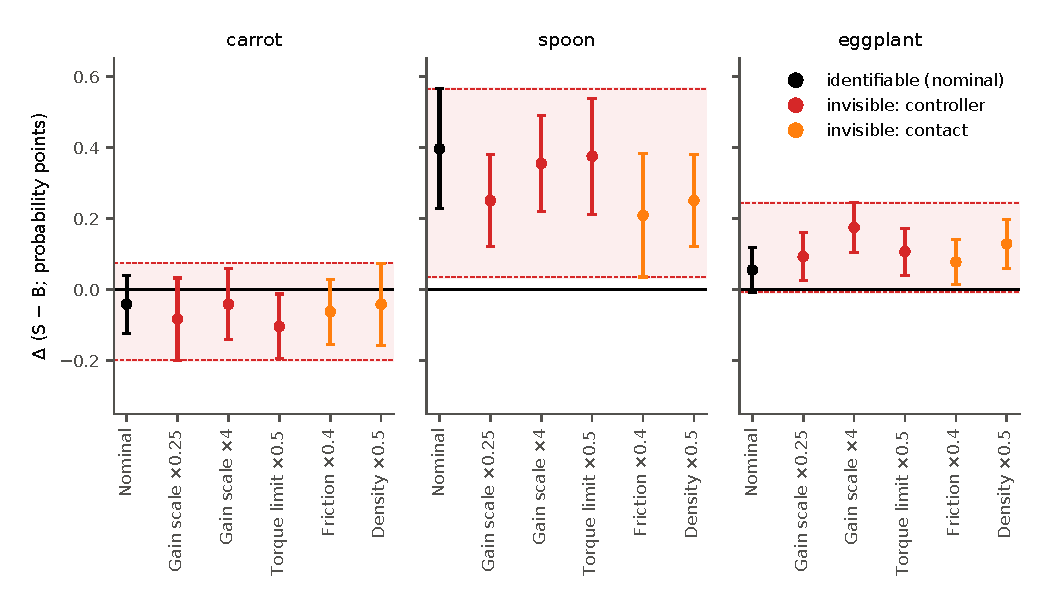
\includegraphics[width=\textwidth]{Fig4}
\caption{Policy differences across simulator conditions}\label{fig4}
\figurenote{S and B denote Octo-Small and Octo-Base, respectively; $\Delta$ is the success rate of S minus that of B on three Bridge tasks. Black points denote calibration-identified conditions; coloured points denote calibration-invisible conditions. Multipliers are relative to nominal; gain scale multiplies arm-joint stiffness and damping equally. Shading is the sampled-set envelope over invisible conditions and nominal. Estimates use runs as observations (Sect.~\ref{subsec7_2}); eggplant has five seed sets, spoon and carrot two. Per-cell configuration and run counts are in Appendix~\ref{secC}.}
\end{figure*}

%%=============================================================================%%
\section{A verdict ladder and its reach}\label{sec8}

Sections \ref{sec4} through \ref{sec7} establish that a simulation benchmark's ranking claims are
underdetermined by the evidence behind them, from three independent directions. This section asks
what to do about it: what a set-valued criterion buys, at what cost in power, and where it stops
working. The tests separate sampled-set validity, model-dependent interpolation, and real-world validity.

\subsection{Two rungs, with different guarantees}\label{subsec8_1}

\textbf{The union envelope} declares an ordering when the interval at every sampled parameter
setting in $F_{\mathrm{nom}}$ supports the same sign. Conditional on the per-setting interval
validity assumed in Sect.~\ref{subsec3_3}, its error bound concerns the finite set of settings
actually evaluated. It does not cover values between them.

\textbf{A Gaussian-process simultaneous posterior band} fits $\Delta(z)$ over the parameter axes
and evaluates posterior functions on a specified grid. We mix draws over a grid of
$(\ell, \sigma_f)$ hyperparameters using marginal-likelihood weights, then take $L$ as the
$2.5$th percentile of the per-draw grid minimum and $U$ as the $97.5$th percentile of the per-draw
grid maximum. This gives a nominal $95\%$ posterior envelope for the grid extrema, subject to
Monte Carlo approximation and conditional on the GP model, likelihood and hyperparameter grid.
It is not a frequentist confidence guarantee or a certified bound on extrema between grid points.

For Fig.~\ref{fig6}, approximately $4{,}000$ draws are evaluated on the points of a
$41\times41$ grid satisfying $|u-v|\le0.25$ and $|u|,|v|\le2$, where $u$ and $v$ are the
base-two logarithms of stiffness and damping multipliers. This nominal-ratio strip is an
exploratory evaluation domain, not the minimiser-based compatible set $C_\alpha$.
The model interpolates between the 13 observed design points; its empirical coverage and power
are assessed separately in Sect.~\ref{subsec8_2}. Mixing over length scales represents uncertainty
that a single fitted length scale would omit, but does not establish that the smoothness model
is adequate.

A flatness gate that chooses between the two criteria per axis was also tested and rejected
for its coverage and false-trigger behaviour (Sect.~\ref{subsec8_2}).

\subsection{Coverage and power on synthetic ground truth}\label{subsec8_2}

Because real data provide no ground truth about $\Delta(z)$, we built a synthetic track in which the
response surface is known and the criteria can be scored directly: 300 repetitions per cell over
four surface families, crossed with true margins $\Delta_0$ and episode budgets $n$.

The synthetic experiment uses $s=(u+v)/2$ and $r=u-v$. Its default domain has $|s|\le2.5$
and $|r|\le0.25$; a separate sensitivity analysis restricts $|s|\le2$.
The GP calculation evaluates approximately 1{,}000 posterior draws per repetition on a
$41\times3$ grid in $(s,r)$. The reference extrema $[L^*,U^*]$ are evaluated on a denser
$81\times5$ grid. Reported coverage therefore concerns these reference-grid extrema;
neither grid supplies a certificate for extrema of an arbitrary continuous surface.

\begin{table*}[t]
\caption{Coverage, error and declarations on synthetic surfaces}\label{tab7}
\begin{tabular}{@{}llll@{}}
\toprule
Surface & Point calibration & Union envelope & GP simultaneous band \\
\midrule
Flat & 0.92 / 0.05 / 0.53 & 1.00 / 0.00 / 0.24 & 1.00 / 0.00 / 0.14 \\
Linear & 0.24 / 0.36 / 0.71 & 0.99 / 0.00 / 0.29 & 0.95 / 0.00 / 0.15 \\
Dip at a sampled setting & 0.00 / 0.88 / 0.45 & 0.98 / 0.00 / 0.03 & 0.97 / 0.00 / 0.04 \\
Dip between settings & 0.00 / 0.85 / 0.43 & 0.22 / 0.17 / 0.21 & 0.91 / 0.00 / 0.08 \\
\bottomrule
\end{tabular}
\tablenote{\textit{Notes.} Entries give minimum coverage / maximum error rate / mean declaration rate. Coverage and error extrema use all cells in each family; declaration rates are averaged only over cells with decidable truth. All methods use the same strip extending beyond the sampled design; narrowing the strip changes the ground truth $[L^*, U^*]$ (Sect.~\ref{subsec8_2}).}
\end{table*}

\paragraph{(i) Point calibration's error rate rises with the episode budget.}
On any non-flat surface the nominal interval covers $\Delta(\hat z)$ rather than the extremes over
the specified synthetic evaluation domain, so more episodes shrink the interval around a
different quantity from the domain extrema being assessed. On the linear surface at $\Delta_0 = 0.1$ the error rate goes from 0.13 at $n = 24$ to
0.36 at $n = 96$; on the sampled-dip surface at $\Delta_0 = 0.2$, from 0.26 to 0.88. This is the
quantitative form of ``more evaluation makes a wrong conclusion more confident''.

\paragraph{(ii) Union-envelope coverage depends on sampling the extrema.}
Where the extremum of $\Delta(z)$ falls on a sampled setting it has coverage $\ge 0.98$ with error
rate 0 and the highest power among the methods meeting the nominal coverage target in these cells (declaration rate 0.98 on the flat surface at
$\Delta_0 = 0.3$, $n = 96$). Where the decisive feature falls between sampled settings it fails
outright: coverage 0.22, error rate 0.17.

\paragraph{(iii) GP-band coverage and the power trade-off.}
Across the four surface families, the GP band's minimum observed coverage is 0.91 and its
observed error rate is 0. These are empirical frequencies over 300 repetitions per cell,
not a coverage guarantee; 0.91 is below the nominal level of 0.95. At 300 repetitions,
the Monte Carlo standard error near coverage 0.9 is about 0.017, placing the 0.91 result
roughly two standard errors below nominal. The shortfall is therefore unlikely to arise from
simulation noise alone. Table~\ref{tab7} assesses the smoothness prior on these four families;
the results do not establish distribution-free validity. On the flat surface at
$\Delta_0 = 0.3$, $n = 96$, the declaration rate is 0.47 and increases little from $n = 48$
to $n = 96$, because the evaluation region extends half a grid step beyond the sampled range
and posterior uncertainty increases at its boundaries.

Narrowing the strip to the sampled range raises that rate to 0.77 and restores monotonicity in $n$,
and it is tempting to adopt it on that basis. We report it as a sensitivity analysis instead,
because the change is not confined to the band. The strip extent enters the ground truth
$[L^*, U^*]$, so narrowing it narrows what every method is asked to cover: point calibration's
maximum error rate on the linear surface falls from 0.36 to 0.04 and the union envelope's mean
declaration rate from 0.29 to 0.19, purely from the redefinition. Comparing the band's 0.91 observed
coverage under one truth against its 0.85 under another is therefore not a like-for-like measurement
of one estimator, and we do not present it as one. Within the narrowed configuration, taken whole,
the band's minimum observed coverage is 0.85 on the between-settings dip with a nonzero
error rate (0.01). This coverage is further below nominal than the headline table's figure, and we attach the
$\ge 0.91$ observation only to the configuration Table~\ref{tab7} reports.

For the empirical simulation data in Fig.~\ref{fig6}, the 13 design points extend to
$|u|, |v| = 2$. Evaluating the band beyond this range would require unsupported extrapolation.
Figure~\ref{fig6} therefore restricts the band to the sampled range.

The highest-weight length scale is $\ell = 0.5$ on all three tasks, with signal scale 0.02 on carrot
and 0.05 on spoon and eggplant, so the band there does not rest on a per-task tuning choice.

One scope limitation has to be stated before Fig.~\ref{fig6} is read alongside anything else in this
paper, because it is easy to miss and it invalidates the obvious comparison. The controller plane
needs 13 design points spanning stiffness and damping independently, and the only sweep we have with
that design uses the older inference-stack build, with 24--96 paired episodes per design point and
per-episode rather than per-configuration standard errors. The main census analyses use the corrected inference build and explicitly stated seed budgets. Fig.~\ref{fig6} is therefore an exploratory
analysis on a different and superseded data scope, not a rung evaluated on the same footing as
the complete-census analysis of Sect.~\ref{subsec7_2}. Supplementary Material S1 gives the
design-point budgets; the two data scopes are not used as
mutual validation. Concretely: on spoon the
GP band over that older sweep declares ($[+0.03, +0.43]$) while the union envelope over the same
older sweep abstains with a lower bound of exactly $0.000$; on the current census
(Fig.~\ref{fig4}) the spoon union envelope is $[+0.04, +0.56]$ and declares. Those three numbers come
from two different data scopes. Only the two computed on the same older sweep directly compare
methods; comparisons with the current census also change the data scope.
What Fig.~\ref{fig6} contributes is a picture of the response surface over a plane no current sweep
covers, including the ratio direction to which the calibration data are sensitive
(Sect.~\ref{subsec4_4}). We use this figure only to characterise that response surface.

We also report a configuration we rejected, because it is a methodological point rather
than a tuning detail. Imposing a lower bound on the GP length scale equal to the sampling spacing
doubles power again (flat-surface declaration 0.22 to 0.40, linear 0.17 to 0.30) but assumes the
surface is smooth at exactly the scale where the dip families are not, and coverage collapses to
0.45--0.83 with error rates up to 0.10. A response-surface method's power can be bought only with
prior assumptions, and the stronger the prior the more brittle the method is to the features it did
not sample. The rejected flatness gate is the same lesson: with 13 design points the GP already
fits the sampled-dip surface, so the gate only lowered coverage on the between-settings surface
(0.91--0.98 to 0.89) and mis-fired on flat surfaces 16--20\% of the time.

\begin{figure*}[t]
\centering
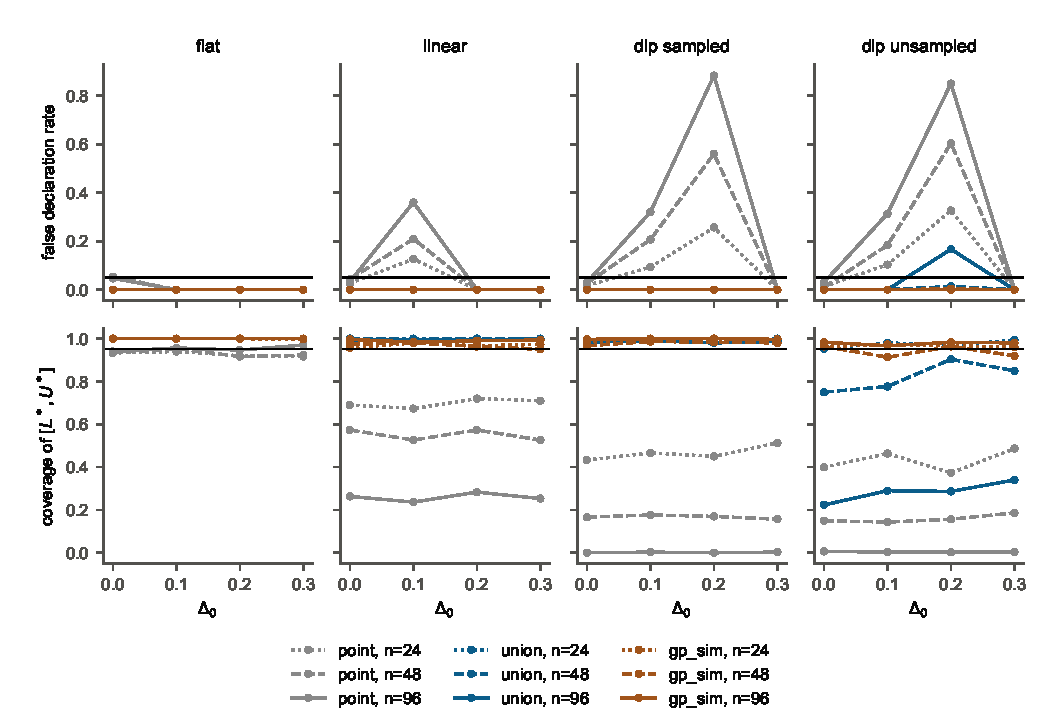
\includegraphics[width=\textwidth]{Fig5}
\caption{Error rates and coverage on synthetic response surfaces}\label{fig5}
\figurenote{Columns: surface families; horizontal axes: true margin $\Delta_0$; line styles: episode budgets. Top: false-declaration rate (nominal 0.05); bottom: coverage of $[L^*, U^*]$ (nominal 0.95). Grey, blue and orange denote point calibration, the union envelope and the GP simultaneous band. Frequencies are empirical over 300 repetitions per cell. Data and strip extent match Table~\ref{tab7}; neither the narrowed-strip variant nor the rejected flatness gate is plotted.}
\end{figure*}

The surfaces in Fig.~\ref{fig6} and the restricted posterior bounds use the same hyperparameter-marginalised model. The bounds use approximately 4{,}000 function draws evaluated on the strip grid defined in Sect.~\ref{subsec8_1}. The bounds are $[-0.10, +0.03]$ for carrot and $[-0.06, +0.36]$ for eggplant, both yielding abstention; spoon has $[+0.03, +0.43]$ and declares Octo-Small better.

\begin{figure*}[t]
\centering
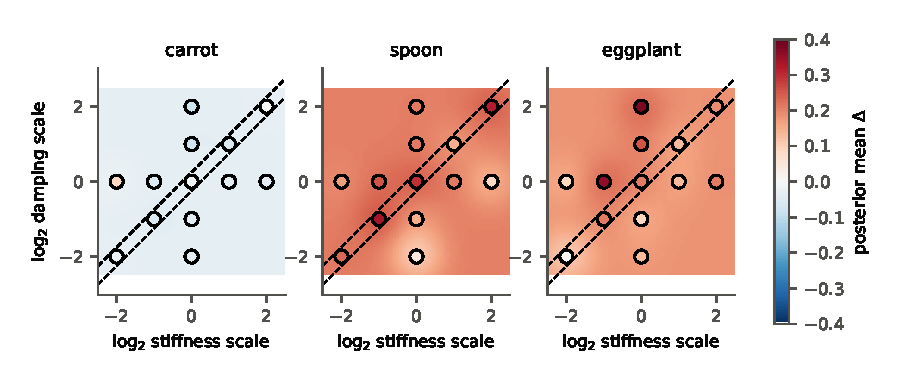
\includegraphics[width=\textwidth]{Fig6}
\caption{Exploratory stiffness--damping response surfaces}\label{fig6}
\figurenote{Posterior mean policy differences after GP hyperparameter marginalisation. Circles: 13 design points; dashed lines: $|u-v|=0.25$, bounding the nominal-ratio evaluation strip defined in Sect.~\ref{subsec8_1}. This strip is not $C_\alpha$. Results use the older inference-stack sweep with 24--96 paired episodes per design point and episode-level standard errors. Budgets are listed in Supplementary Material S1. This exploratory scope is not directly comparable with the census in Fig.~\ref{fig4}; see Sect.~\ref{subsec8_2}.}
\end{figure*}

\subsection{Verdict stability under empirical re-evaluation}\label{subsec8_3}

The synthetic tests do not establish how closely the four surface families represent empirical
simulation responses. We therefore also examine repeated evaluations, defining a verdict as
\emph{stable} when a second evaluation of the same policy pair returns the same verdict.
Some comparisons vary only the policy seed set; others also vary the simulator port or
inference-stack build, which can affect results (Sect.~\ref{subsec5_5}). The analysis measures
consistency across these changes in seed, implementation and protocol. It is not a set of
independent statistical replications under identical conditions.

Each re-evaluation pair enumerates the same configuration grid on both sides. Six of the eight pairs compare the same four Octo variants on eggplant and share policy data; the remaining two are on spoon and carrot. The eight pairs therefore span three tasks and are not independent experiments.

\begin{table*}[t]
\caption{Ranking stability under empirical re-evaluation}\label{tab8}
\begin{tabular}{@{}lrrrrrrr@{}}
\toprule
 & & & & & & \multicolumn{2}{c}{Declaring pairs} \\
\cmidrule(l){7-8}
Criterion & Pairs & Stable & Contradict & Unsupported & Declare & $n$ & replicated \\
\midrule
Point calibration & 8 & 0.50 & 0.00 & 0.50 & 0.38 & 5 & 1 (0.20) \\
Union envelope, controller & 8 & 0.88 & 0.00 & 0.12 & 0.06 & 1 & 0 (0.00) \\
Union envelope, all axes & 8 & 1.00 & 0.00 & 0.00 & 0.00 & 0 & n/a \\
\bottomrule
\end{tabular}
\tablenote{\textit{Notes.} Exploratory analysis of older inference-stack sweeps: 48 episodes per condition and episode-level bootstrap, rather than the current census. Stable includes agreement to abstain. Of the eight non-independent pairs, $n$ counts those declaring on at least one evaluation; replicated counts those declaring the same ordering on both, with the fraction among $n$ in parentheses.}
\end{table*}

Stability increases from 0.50 to 0.88 to 1.00, but this metric includes agreement to abstain.
The all-axes envelope reaches 1.00 because it makes no declaration on these data, so perfect
agreement here provides no ordering information. For the controller-axis envelope, the 0.88
stability comprises seven abstain--abstain agreements out of eight comparisons. Its sole
declaration does not recur in the second evaluation.

The union envelope produces more consistent abstentions. Point calibration declares on five
of eight pairs; for four of those five, it declares in one evaluation and abstains in the other.
The union envelope converts all four into consistent abstentions, reducing the unsupported rate
from 0.50 to 0.12. This does not establish more reproducible declarations. The replication counts
(0 of 1 for the envelope and 1 of 5 for point calibration) are insufficient to compare declaration
reliability. The eight comparison pairs span three tasks, six share policy data, and all use the
older data scope. Coverage is assessed separately against synthetic ground truth in
Sect.~\ref{subsec8_2}. Table~\ref{tab8} shows the empirical trade-off: agreement increases
from 0.50 to 0.88 while the declaration rate decreases from 0.38 to 0.06.

\subsection{Opposite real and simulated mean orderings}\label{subsec8_4}

The preceding tests assess statistical coverage and verdict stability within simulation;
they do not validate real-robot orderings. We examine this distinction using published
real-robot and simulated rates for a selected policy pair. The case uses information available
during development and is not a held-out validation test.

The SIMPLER reference implementation publishes real-robot and simulated success rates for the
same policies on the same task \citep{li2024simpler}. Auditing all of them, 62
within-task policy pairs have both rates published once RT-2-X is excluded for lack of public
weights, and 5 of the 62 have opposite mean directions in simulation and reality, with a
further 3 tied in at least one domain. The selected case is therefore one of several directional disagreements. RT-1 (Converged) denotes the checkpoint trained to convergence, and RT-1 (15\%) denotes the checkpoint at approximately 15\% of the training steps. We study these checkpoints on
Coke-can grasping for three stated reasons: both checkpoints are public, it is on
the embodiment and task where we ran a complete 300-configuration census, and simulation declares it
with a clear margin ($+0.147$). Its published real margin is the smallest of the five: the five real margins are $0.333$,
$0.185$, $0.167$, $0.148$ and, for this pair, $0.067$. The small margin makes real-evaluation uncertainty particularly relevant to its interpretation. These are reasons of convenience
and coverage, not of significance. The
five are directional disagreements between rounded published means, with no per-cell trial
counts and no intervals on either side, so none of them is an established reversal.

Our simulated success rates differ from the published simulated rates by $+0.006$ and $+0.007$ for RT-1 (Converged) and RT-1 (15\%), respectively, preserving the published direction of the difference (Table~\ref{tab9}).

\begin{table*}[t]
\caption{Published and reproduced RT-1 success rates}\label{tab9}
\begin{tabular}{@{}lrrr@{}}
\toprule
Source & RT-1 (Converged) & RT-1 (15\%) & Margin \\
\midrule
Published real robot & 0.853 & 0.920 & $-0.067$ (15\% checkpoint higher) \\
Published simulation & 0.857 & 0.710 & $+0.147$ (converged checkpoint higher) \\
Our nominal census & 0.863 & 0.717 & $+0.147$ \\
\bottomrule
\end{tabular}
\tablenote{\textit{Notes.} Coke-can grasping task. Margin is RT-1 (Converged) minus RT-1 (15\%). Published rates are rounded point estimates without trial counts or intervals; opposite mean directions do not establish a reversal of the true ordering.}
\end{table*}

The question is whether the union envelope abstains on a pair where the simulator's ordering
disagrees with the published real one. It is the sharpest test of the criterion available to us,
because here there is an external number to disagree with. That number is a point estimate
without an interval, a limitation we return to below. We ran both checkpoints over the complete
300-configuration census under nominal conditions plus two calibration-invisible conditions (the
torque limit and object friction), for 1{,}800 episodes total.

One caveat about that choice of conditions belongs here rather than in a footnote. The replay
evidence of Sect.~\ref{subsec4_3} is on WidowX BridgeData demonstrations, and this experiment
is on the Google Robot embodiment. We carried the two conditions over because they are the ones that
moved verdicts on bridge, not because they are established as calibration-invisible for this arm: we
have no Google Robot replay set, so for this embodiment ``calibration-invisible'' is an assumption
imported from the other, and the friction axis is in any case unobserved by free-space replay on
either. The experiment should be read as a test of the criterion's behaviour on a pair with external
real-robot point estimates, not as a propagation of a verified compatible set.

The result is adverse. Point calibration on the nominal condition gives $[+0.083, +0.210]$, declaring
RT-1 (Converged) better. The union envelope over the two dynamics conditions gives
$L = +0.070$, $U = +0.240$, also declaring RT-1 (Converged) better, which is opposite to the
ordering of the published real-robot point estimates.

Widening from the point to the set moved the lower bound from $+0.083$ to $+0.070$, so the shift
that would reach abstention is $0.070$: the bound has to lose that much on its lower end, not the
$0.214$ separating the simulated margin from the real one. Measured against $0.070$, the two dynamics
conditions are not close: their margins span 0.133 to 0.177, a spread of 0.044, which is less than
the distance to zero. But that is a statement about these two conditions, not about hidden
variables in general, and the distinction matters: across the twelve texture $\times$ condition cells
the margins span $+0.053$ to $+0.213$, a spread of $0.160$, more than twice what abstention requires.
The axis that carries no physics has the range to move this verdict; the two dynamics parameters do
not.

Having the range to move the verdict is not the same as rescuing the criterion, however, and on
inspection it does not. Because this run puts a second policy on
the same 300-configuration grid, it also settles the question left open by Sect.~\ref{subsec5_5}:
whether a visual variant that carries no physics can flip a ranking rather than merely
inflate a single policy's variance. Adding robot texture variant as a fourth set dimension (12 cells
of 75 configurations each) does turn the verdict to abstention, $L = -0.067$, but the abstention
is of the second kind identified in Sect.~\ref{subsec7_5}. All twelve cells have positive
point margins, from $+0.053$ to $+0.213$, and none of the cell-specific intervals supports a higher success rate for RT-1 (15\%) than for RT-1 (Converged). The bound reaches zero only through interval width at
75 configurations per cell.

The asymptotic interpretation requires an additional assumption. Each cell's interval is a policy-noise interval over an enumerated 75-configuration sub-grid, so its
width shrinks with additional runs per configuration rather than with additional episodes. If
the twelve observed point margins were the population quantities, $L$ would tend to their minimum,
$+0.053$, and the abstention would dissolve. But they are not: with one run per configuration each
cell margin carries binomial uncertainty we have not resolved, so twelve positive sample
means do not establish that all twelve population means are positive, and $+0.053$ is where the
bound tends under our estimand rather than a measured endpoint. What we can say without that
assumption is narrower and enough for the purpose: the abstention here is produced by interval width
and not by any cell disagreeing in sign, so by our own test in Sect.~\ref{subsec7_2} it is at least
partly our power rather than a demonstrated parameter fact, and we decline to claim it as a success
of the criterion. Resolving whether it is only power would need repeat runs per configuration
in each cell, which we have not done.

The published real margin, $-0.067$, is comparable in magnitude to the policy-seed noise
measured in simulation, and the published real rates have no uncertainty intervals.
The opposite mean directions may therefore reflect real-evaluation noise or a model gap.
If they reflect a model gap, the simulated declaration is incorrect for the robot; if they
reflect measurement noise, the real evaluation does not resolve the pair. Neither explanation
allows the simulated declaration alone to establish the real-robot ordering.

The conclusion we draw is therefore about the criterion's reach, and we bound it to what was
actually tested. The difference between the simulated margin and the published real one is $0.214$,
and one policy's own rate differs by $0.203$ (RT-1 (15\%): 0.920 real against 0.717
simulated). Against that, abstention on this pair would have required the union's lower bound to
lose $0.070$. The three dynamics cells we ran span $0.044$ and do not reach it; the twelve
texture $\times$ condition cells span $0.160$ and do reach it, though only by interval width and
without any cell changing sign. The result has three scope boundaries. Within the settings
we ran, no configuration of the calibration-invisible parameters produces the real robot's
ordering. Beyond them we do not know: we tested two dynamics conditions at one value each and
one visual axis at its four values, out of a parameter family that is continuous in friction,
density, the common gain scale and the torque limit, and we did not explore interactions. And the
comparison target is a point estimate: the published real rates come without intervals, so the
$0.214$ is a difference between one number with an interval and one without.

Under the tested conditions, the declared ordering is opposite to the ordering of the
published real-robot point estimates. Attributing this discrepancy to effects outside the
entire parameter family constrained by demonstration replay would require broader parameter
coverage or real-robot replication with quantified uncertainty. Neither is available here.
Under the conditions in Sect.~\ref{subsec3_4}, the discrepancy is consistent with a potentially
large $b_{ij}$ that a criterion based only on $E_\theta$ and $E_{MC}$ cannot identify.

\subsection{What the ladder is for}\label{subsec8_5}

Together, the tests delimit what the criteria measure. The sampled-set envelope bounds extrema
over evaluated settings; in the synthetic tests it has conservative observed coverage when the
extrema are sampled and fails on the between-settings dip. The GP band addresses interpolation
under its smoothness prior but undercovers in some tested cells (Sect.~\ref{subsec8_2}).
On empirical re-evaluations, the sampled-set envelope abstains consistently where point calibration
declares on one replicate and not the other, which is a claim about abstention and not about
declarations (Sect.~\ref{subsec8_3}); and it changes the verdict on 3 of 17 bridge policy pairs at
the reference protocol's three seed sets, falling to 1 of 17 at five seed sets over a full census
(Sect.~\ref{subsec7_2}). Both counts are uncorrected for multiplicity across pairs; under Holm the
rules disagree on 4 of 17 rather than 1, because the correction removes more of the envelope's
declarations than of point calibration's (Sect.~\ref{subsec7_2}). Which count to quote depends on
whether the claim is about one named pair or about whichever orderings the table declares, and the
extra abstentions are abstentions rather than demonstrated corrections. It does not bound, and cannot bound, the ambiguity arising from a model gap
that no setting of those parameters expresses. Sect.~\ref{subsec8_4} exhibits a pair where
reaching abstention would have needed 0.070 while the gap between the simulated and published real
margins is 0.214 and points the other way.

These results support using the union envelope to identify cases in which the benchmark's
evidence is insufficient to determine an ordering (Sects.~\ref{subsec8_2} and~\ref{subsec8_3}).
They do not establish it as a rule for selecting the better real-world policy. A declaration
remains conditional on the evaluated parameter set and does not provide a sim-to-real
guarantee; the comparison in Sect.~\ref{subsec8_4} motivates external validation.

%%=============================================================================%%
\section{Limitations}\label{sec9}

The limitations below distinguish the breadth of the empirical evidence from the assumptions
needed for statistical or real-world guarantees.

\begin{enumerate}
\item \textbf{The operating-point measurement covers two tasks and one policy pair.}
Section~\ref{subsec4_4} finds that the replay loss over our grid is minimised at
$(k{\times}2, d{\times}0.5, \text{delay}\ 1)$ on both stacks, and that nominal (ratio 1, no delay,
where the reference benchmark computes its published rates) is rejected against that minimiser on our 98
demonstrations. Sect.~\ref{subsec4_3} states why that is a re-calibration result and not a claim
about the original fit: we did not verify that our demonstrations are the trajectories that fit
used, and our search grid may be wider than its.
Section~\ref{subsec7_7} measures the resulting evaluation changes using complete censuses on two tasks. This covers two tasks, one
policy pair and one alternative operating point. The two tasks show different changes in the set
verdict, but do not establish which behaviour is typical or which task properties explain the
difference. The spoon result is also the stronger
of the two, and a reader should weigh that it rests on a 24-configuration grid at two seed sets
rather than 64 at three, so its block interval carries one degree of freedom. Further evaluation
should include carrot, more policy pairs and another alternative operating point, so that the
fitted setting is not the only contrast.

Within each task, the planned design is complete. Each of the two operating points on each task carries a full six-condition
fibre (24 complete configuration censuses across the two tasks), and fibre membership at
the fitted ratio is measured rather than assumed: the replay grid varies the common scale at seven
other ratios but only once at $0.25$, so we swept the scale sixteenfold at ratio $0.25$ directly and
re-measured the torque limit at the fitted gains; its nominal-point status cannot be assumed because the
fitted point doubles the stiffness (Sect.~\ref{subsec7_7}). What is narrow here is the number of
tasks and pairs, rather than completion of the planned design within each task.

\item \textbf{The criterion's central negative result rests on one selected policy pair.}
Section~\ref{subsec8_4} shows the union envelope declaring an ordering the published real means
reverse, on one pair, one task, one embodiment. It is not the only such pair: our audit of the
published tables finds 5 of 62 within-task pairs with opposite mean directions, and we chose this one
for public checkpoints, census coverage and a clear simulated margin, not for the size of its
real margin, which is the smallest of the five. This case was selected using development
information. It illustrates the criterion's limited scope, rather than estimating the frequency
of such disagreements or providing a held-out test. The four other pairs are identified in the
audit, and one of them
(Octo-Base versus Octo-Small on carrot) is a bridge pair we already have a census for.
A union envelope declaration therefore supplies no guarantee of real-world ordering; this selected
case does not establish how often such declarations disagree with reality.

\item \textbf{No hardware of our own.} Every simulated number here is ours; every real-robot number
is quoted from the reference implementation's published tables. Those are the values the benchmark
itself is validated against, and using them is what makes Sect.~\ref{subsec8_4} possible without a
laboratory, but they carry their own uncertainty and are published without intervals: they are
single-protocol real
evaluations, and the pair in Sect.~\ref{subsec8_4} has a real margin of 0.067, of the same order as
the seed noise we measure in simulation.

The following prospective protocol would test whether the ordering our
criterion declares on RT-1 (Converged) versus RT-1 (15\%) holds on the robot; the
published point estimates point the other way, but they carry no interval, so they do not establish
an erroneous declaration. The design would evaluate those two checkpoints on
Coke-can grasping, on hardware matched to the published protocol in the respects that decide an action:
the same arm, the same control interface and action semantics, the same camera placement and the
same scene layout. A different 7-DoF arm is not a replication of this benchmark merely by
having seven joints.

Planning this comparison requires statistical power as well as interval precision. Suppose the
published rates $0.853$ and $0.920$ are the truth, trials are independent Bernoulli, arms are
equally sized, and there is no scene clustering or protocol drift. All four assumptions are
optimistic. Table~\ref{tab:power} reports the resulting precision and power for a two-sided
normal-approximation test at $\alpha = 0.05$.

\begin{table}[h]
\caption{Prospective precision and power for robot trials}\label{tab:power}
\centering
\begin{tabular}{@{}rrrr@{}}
\toprule
per policy & total & expected half-width & power \\
\midrule
200 & 400 & 0.062 & 0.57 \\
400 & 800 & 0.044 & 0.85 \\
800 & 1{,}600 & 0.031 & 0.99 \\
\bottomrule
\end{tabular}
\tablenote{\textit{Notes.} Independent, equally sized Bernoulli samples with success probabilities 0.853 and 0.920; two-sided normal approximation at $\alpha=0.05$. These are optimistic planning estimates, not a formal sample-size determination.}
\end{table}

\noindent Thus $n = 200$ per policy provides only modest power: an expected half-width of $0.062$
below a hypothesised gap of $0.067$ does not ensure that an observed interval excludes zero. About
$400$ per policy ($800$ trials in total) is the point at which the hypothesised gap would be detected
$85\%$ of the time. A paired design, clustering, a different true gap or a different stopping
rule all move these figures, so the table provides an indicative trial budget under the stated
assumptions. A definitive sample-size determination requires specifying the final experimental design.

Two choices should be fixed before the trials start: the analysis rule (interval, threshold and
observation unit) and the simulator operating
point against which the comparison is made. Our release contains the simulated side at census scope,
so the real side is the only missing term. The four other pairs with opposite published
real and simulated mean directions in the 5-of-62 audit of
Sect.~\ref{subsec8_4} extend the same design at the same cost per pair, and one of them
(Octo-Base versus Octo-Small on carrot) is a bridge pair for which we already
hold a complete configuration census, so new data collection is needed only on the real robot.

This remains a proposed protocol: we have no arm, and the two public evaluation services
that would have supplied one were unavailable during this work (Sect.~\ref{subsec1_3}). A reader
with access to suitable hardware can use the released checkpoints, settings and analysis protocol
to conduct this validation.

\item \textbf{One suite, and two kinds of conclusion.} Every measurement here comes from a single
evaluation suite. Claims that follow from construction apply to benchmarks satisfying the same
assumptions: that an
index-driven initial state makes the configuration set a finite population rather than a sample;
that the analysed controller formulation and free-space excitation can leave common gain scaling and
an inactive saturation limit unconstrained; and that a criterion over a compatible set bounds only
the ambiguity represented by that set. These arguments depend on their stated construction and
excitation conditions. The magnitudes are specific to this instance and should not be
extrapolated: a mean of 0.121 for the
torque shift, 0.400 for the texture spread, 1 of 17 disagreeing pairs, and the 0.038 reproduction. A
reader should distinguish mechanisms that extend under the same assumptions from measurements
showing that their effects can be substantial in this suite.

\item \textbf{Narrow coverage of policies, embodiments and tasks.} The principal policy comparisons
use seven configurations from three families: four Octo configurations (small and base, each with
default and single-frame history), one OpenVLA configuration and two RT-1 checkpoints. The audit
covers two embodiments and five tasks: four Bridge tasks in the reference-protocol reproduction
and Coke-can grasping in the Fractal comparison. The main Bridge sensitivity censuses cover three of
those tasks. OpenVLA is run 4-bit quantised, which we did not control against a bfloat16 baseline; the
torque mechanism in Sect.~\ref{subsec7_4} is a claim about the quantised model as deployed. The
dependence of decision-relevance on the task-policy pair limits extrapolation: an effect can be
substantial on one task and nearly absent on another, and
we cannot say which is typical.

\item \textbf{No resolved strong-form reversal was observed in the evaluated settings.} No
calibration-invisible parameter reverses a sign-determined ranking in these measurements. The
negative density-cell estimate at the smaller budget also does not persist at five seed sets
(Sect.~\ref{subsec7_5}); the remaining near-zero estimates do not establish a resolved reversal.

\item \textbf{The fibre is sampled, not covered.} The union envelope evaluates a discrete set of
parameter settings, so its coverage statement concerns extrema over those settings only.
Section~\ref{subsec8_2} shows that extending this interpretation to the continuous region can fail
(observed coverage 0.22) when the decisive feature lies between sampled
settings. Concretely, we sample the common scale at $\times\tfrac14$ and $\times 4$, the torque
limit at $\times\tfrac12$, and friction and density at one value each. These five points stand in
for a region that is continuous in four coordinates, with no interactions explored. On the contact
axis three sampled points are too few for the GP rung to be trustworthy, so those axes use the union
bound and inherit its limitation.

\item \textbf{Limited replication contributes to abstention.}
Several tasks sit at success rates of 0.1 to 0.5, where even a complete 24-configuration census at
three seeds gives half-widths of 0.05 to 0.13. We applied the $h \to 0$ test wherever the budget
allowed. For policies with only one independent run per configuration, including original-stack
OpenVLA and the RT-1 comparison, run-to-run variation cannot be estimated empirically; the
complete per-pair table identifies the variance model used. Original-stack Octo-Small and
Octo-Base instead have two runs per configuration in the main sensitivity censuses.

\item \textbf{Implementation-build drift is separated on two policies only.} The $-0.109$ shift and
the 0.73--0.88 episode-level agreement come from a single controlled re-run of two Octo policies
across two inference-stack versions, with one run of each build. The figure therefore carries no seed
replication and no interval. This supports treating $\pi$ as a separate evaluation axis, although
the evidence is more limited than for the other effects in Sect.~\ref{sec5}.

\item \textbf{Part of the platform work is exploratory.} The ManiSkill3 configuration was used for
the sweeps, with the original reference stack used for cross-checking. Both show sub-millimetre
replay insensitivity over the tested ranges. Under the current run-unit analysis, the point and
sampled-set verdicts agree for Octo-Small versus Octo-Base on the three shared Bridge tasks,
although the estimated policy gaps differ. Their eggplant configuration grids also differ, so
per-episode comparison is undefined there. Rows are labelled by stack throughout and should not be pooled.
\end{enumerate}

%%=============================================================================%%
\section{Conclusion}\label{sec10}

This audit connects three properties of a robot-policy evaluation protocol to the comparisons it
supports: the dynamics excited by calibration, the configuration population being evaluated, and
the budget and analysis used to estimate a policy difference. They require different remedies.
Additional independent runs reduce policy randomness, but repeated evaluation at one simulator
setting does not measure sensitivity to other settings or to a different configuration population.

The measurements make this distinction concrete. Replay of 98 demonstrations leaves common gain
scaling and an inactive torque limit weakly constrained over the tested ranges. On a fixed
ManiSkill3 eggplant census, one pair's estimated gap ranges from 0.055 to 0.174 across conditions;
the separate replay bounds in Table~\ref{tab6a} come from the original ManiSkill2 stack. Reapplying
the calibration protocol to same-source demonstrations favours a different controller operating
point on both stacks. Complete censuses at that point change the single-setting declaration on both
tasks measured, with different consequences for the set rule: on eggplant the point rule moves
from abstention to declaration, although the paired change in the policy gap is $+0.031$ and
unresolved and both set envelopes abstain; on spoon the paired change is
$-0.271$, resolved under every sampling model we report, and it withdraws a declaration that both
rules supported at the shipped setting. The two tasks demonstrate that a sampled-set declaration
can depend on the operating point. This establishes sensitivity under
the stated protocol, not an error in the original parameter fit.

The finite configuration grids contain 24 to 300 states, and two ports can enumerate different
populations. A census therefore removes configuration sampling error for its stated population,
not policy randomness or deployment uncertainty. At the published 72-episode budget, one or two
of four reported orderings are resolved, depending on the variance model. Across 17 bridge pairs
at their released budgets, Holm-adjusted single-setting and sampled-set analyses retain nine and
five declarations respectively. The four additional abstentions quantify sensitivity to the sampled
parameter set under the inference assumptions; they are not verified corrections of real-world errors.

These findings motivate a compact reporting protocol. Specify the configuration population, visual
aggregation, simulator and inference builds, observation unit, policy-randomness lifecycle and
replication budget. Report the controller setting used for the rates, its loss on the stated
calibration data, and the best loss found over an explicit search domain. A setting away from that
minimum may be justified by stability, runtime or evidence outside the replay set; reporting these
quantities makes the choice inspectable. Use independent policy replicates to address unresolved
sampling uncertainty, and separate parameter-sensitivity analysis to assess dependence on modelling
choices. A set-valued declaration describes only the finite settings examined. Published real-robot
point estimates motivate further validation, but neither those means nor our simulation audit supply
a guarantee of real-world policy ordering.

%%=============================================================================%%
\section*{Use of generative AI}

Large language models (OpenAI ChatGPT/Codex) assisted with manuscript revision, analysis scripts. Quantitative results are computed from the recorded episodes by the supplied
scripts. The authors are responsible for the study design, verification and interpretation of the
results and the final manuscript; no language model is listed as an author.

%%=============================================================================%%
\begin{appendices}

\section{Test inversion for the compatible set}\label{secA}

\subsection{Construction}\label{secA1}

Calibration observes $M$ real demonstrations. For a candidate parameter $z$, let $L_m(z)$ be the
replay error on demonstration $m$ (the deviation between the simulated and recorded trajectories),
and let $\hat z$ minimise $\bar L(z) = M^{-1}\sum_m L_m(z)$ over the grid we search.

In addition to reporting $\hat z$, we construct an empirical set by inverting a one-sided test.
For each candidate $z$ we form the paired
per-demonstration differences $\{L_m(z) - L_m(\hat z)\}_{m=1}^{M}$, resample demonstrations with
replacement $B$ times, and take $\mathrm{lo}_{1-\alpha}(z)$ to be the $\alpha$ quantile of the
bootstrap distribution of their mean. Then
\begin{equation}\label{eq:csetA}
C_\alpha = \big\{ z : \mathrm{lo}_{1-\alpha}(z) \le 0 \big\},
\end{equation}
the set of parameters whose replay error is not rejected as worse than that of the selected
minimiser. The selection caveat in Sect.~\ref{subsec3_2} prevents interpreting this empirical set
as a confidence set. Pairing controls for differences in demonstration difficulty that would
otherwise contribute to the variance of the comparison.

The threshold in Eq.~\eqref{eq:csetA} is exactly zero, with no equivalence margin, so any
strictly positive lower bound rejects, however small it is. We apply this choice consistently:
Sect.~\ref{subsec4_4} reports that it
rejects the simulator's own nominal setting on both stacks. The companion analysis
makes the search domain, the loss, $\alpha$ and an optional margin $t \ge 0$ explicit, and
prints the margin that would be needed to retain any given candidate, so that if a future version of
this analysis uses an engineering-equivalence tolerance, that tolerance can be explicitly stated
and justified.

The following properties support the argument of Sect.~\ref{sec4}.

\paragraph{Separation between insensitive and identified directions.}
The two comparisons used in this paper have distinct purposes. The set construction of
Eq.~\eqref{eq:csetA} tests candidates against the grid's
loss minimiser, and under that test nominal is rejected (Sect.~\ref{subsec4_4}). The figures
below are a different and narrower comparison: each insensitive direction against nominal,
which measures the flatness of the loss along that direction and says nothing about whether nominal
itself is retained by the set construction. The following measurements characterise the
directions through nominal, which the minimiser-based test rejects.

If $L_m(z) = L_m(z')$ for every $m$, the paired differences vanish identically, the bootstrap
distribution is a point mass at zero, and $\mathrm{lo}_{1-\alpha} = 0 \le 0$ irrespective of $\alpha$,
$B$ or $M$. Our two directions approach that limit rather than attaining it, so what matters is the
measured margin. Tested against nominal on the 98 demonstrations:

\begin{itemize}
\item \emph{Common gain scaling.} On ManiSkill3, over the fourfold range $\times 0.5$ to $\times 2$
at fixed ratio and delay, the absolute paired mean loss differences are at most $3.3\times10^{-7}$,
with $95\%$ interval lower bounds no lower than $-5.6\times10^{-7}$. Retained.
\item \emph{Torque limit halved.} The paired mean loss difference is $-1.1\times10^{-10}$ on
ManiSkill3 and $-1.8\times10^{-8}$ on the original stack, with exactly one of 98 demonstrations
contributing a nonzero term on each. Retained.
\end{itemize}

\noindent For comparison, the identified directions are rejected with lower bounds of
$+1.5\times10^{-3}$ to $+2.2\times10^{-3}$ (Sect.~\ref{subsec4_4}). Every loss figure in this
appendix is in the composite units of Eq.~\eqref{eq:loss}, which adds metres to radians and is
therefore not a length. The separation between
``retained'' and ``rejected'' here is four to seven orders of magnitude. This large numerical
separation supports the distinction at the reported analysis settings, but does not make the
reference choice immaterial. Section~\ref{subsec4_4} shows that comparisons against the grid
minimiser can reject the nominal point despite the local flatness along the insensitive
directions.

\paragraph{Unobserved parameters are compatible for a different reason.}
Contact friction and object density never enter a free-space replay trajectory at all, so their
compatibility reflects the protocol's coverage rather than its precision. We flag these
separately throughout, because a reader might otherwise conclude that a longer or better-excited
free-space demonstration set would constrain them. A protocol involving contact is needed.

\paragraph{Identified directions are excluded with margin.}
Along the gain ratio and the execution delay the same procedure returns strictly positive lower
bounds. Relative to nominal, ratio $\times 0.5$ and $\times 2$ raise the mean paired loss by
$+0.0064$ and $+0.0089$ (Sect.~\ref{subsec4_3}); relative to the grid minimiser, nominal itself is
rejected at $+0.0022$ on ManiSkill3 and $+0.0015$ on the original stack
(Sect.~\ref{subsec4_4}). Thus the construction is not vacuously inclusive: it excludes
substantively different settings and, on these data, also excludes the shipped setting.

\subsection{Conditions for a real-world ordering guarantee}\label{secA2}

Writing $[L_{ij}, U_{ij}]$ for envelope bounds over the settings and builds under consideration,
the claim that
simulated ordering extends to real-world performance can be justified through the following three
sufficient events:
\begin{align}
E_\theta &= \{ z^* \in S \}, \\[2pt]
E_{MC}   &= \big\{ \forall z \in S,\ \forall \pi \in \Pi,\ \forall (i,j): \notag \\
         &\qquad L_{ij} \le \Delta^{\mathrm{sim}}_{ij}(z; \pi)
                 \le U_{ij} \big\}, \\[2pt]
E_b      &= \big\{ \forall (i,j):\ |\Delta^{\mathrm{real}}_{ij} -
             \Delta^{\mathrm{sim}}_{ij}(z^*)| \le b_{ij} \big\},
\end{align}
Here $\Delta^{\mathrm{sim}}_{ij}(z^*)$ in $E_b$ refers to a specified reference build in $\Pi$.
On $E_\theta \cap E_{MC} \cap E_b$ every real difference lies in
$[L_{ij} - b_{ij},\ U_{ij} + b_{ij}]$ simultaneously, and if those events hold at levels
$1-\alpha$, $1-\gamma$ and $1-\beta$, a union bound gives at least $1 - \alpha - \beta - \gamma$
without any independence assumption. We write the levels conditionally because none of the three is
established here. The caveats below apply; in particular, our $S$ carries no coverage
guarantee at all. Note that $E_{MC}$ is stated over $\Pi \times S$: the implementation build is
treated as an axis of the same kind as the physical parameters, for the reason given in
Sect.~\ref{subsec5_5}.

Each event requires separate justification. The following five qualifications distinguish
the sufficient conditions above from the guarantees supported by the measurements.
The first two identify requirements that remain unmet.

\begin{enumerate}
\item \textbf{Neither set we use carries a coverage probability, and for two separate reasons.}
The first is the selection effect of Sect.~\ref{subsec3_2}: $C_\alpha$ as computed picks its
reference from the same demonstrations it then tests on, and under a null of equal-risk candidates
at our $K$ and $M$ that retains a true minimiser about $53\%$ of the time rather than $95\%$. Thus
even $C_\alpha$ is an empirical rule, not a confidence set; a split-sample variant recovers most of
the level and we report it, but we do not claim exactness for it either. The second is that our
verdicts do not range over $C_\alpha$ at all but over the invisible fibre through nominal
(Sect.~\ref{subsec4_4}), which is generated by a point the calibration data reject. On both counts
$P(E_\theta)$ is unknown for the sets used here. The real-world guarantee therefore remains
conditional on the benchmark's operating point and on probability levels not established in this study.

\item \textbf{Our intervals are per pair; $E_{MC}$ and $E_b$ are joint events.} We compute an
interval for each policy pair separately and report the collection. Such marginal statements
do not establish $\forall (i,j)$; simultaneous inference requires a multiplicity adjustment.
Sect.~\ref{subsec7_2} reports the effect of Holm adjustment: point
calibration falls from 11 declarations to 9, and the union envelope from 10 to 5. The marginal bounds
of $+0.0091$ and $+0.0095$ are among the declarations it removes.
These corrected counts provide a family-wise statement for the 17 pairs, whereas $E_{MC}$
also quantifies over $\Pi \times S$. They therefore do not establish the full joint event.
Our per-pair results should be read as exploratory in the multiplicity sense. This is a statement
about multiple policy pairs, not about the envelope over conditions: for a fixed finite set
of conditions the probability of a false declaration in either direction is at most
$2\alpha_1 = 0.05$, conditional on valid per-setting tail bounds, without an additional correction
across conditions. The argument in Sect.~\ref{subsec3_3} bounds each pre-specified direction by
$\alpha_1 = 0.025$: a wrong positive declaration requires one particular condition's lower bound
to exceed its truth, and the opposite direction has a symmetric upper-tail event. The two multiplicities are different: across conditions the
error event identifies a particular interval that must fail; across policy pairs it does not.

\item \textbf{$E_\theta$ presumes that $z^*$ exists.} The event is empty of content if no
parameter setting reproduces reality, that is, if the simulator is structurally misspecified
rather than merely uncalibrated. Fitted parameters may then be only locally effective quantities,
and $\alpha$ supplies no real-world coverage bound. Section~\ref{subsec8_4} illustrates the need
to examine this premise: none of the sampled settings reproduces the ordering of the published
real means. Without intervals for those means, this disagreement does not distinguish structural
misspecification from real-evaluation uncertainty.

\item \textbf{A Gaussian-process posterior standard deviation is not $\gamma$.} Substituting the
posterior spread of the response-surface rung into $\gamma$ without validating its calibration
would assume the very smoothness the rung is there to test. Section~\ref{subsec8_2} measures that
rung's coverage on synthetic surfaces instead, including surfaces that violate its prior.

\item \textbf{Surrogate error must be bounded to be absorbed.} Where an approximation has a
certified error bound, the band can be widened by it. Where it does not, that rung is an empirical
diagnostic and must not be reported as a coverage guarantee.
\end{enumerate}

Two further points concern variance reduction rather than coverage. Pairing on common initial states
and common exogenous random draws can reduce the variance of $\hat\Delta$ when it induces
positive covariance, and we use matched initial configurations throughout,
but it does not by itself produce a simultaneous band over $F_{\mathrm{nom}}$. Simultaneity has to be
constructed, not inherited from pairing. Matching numerical seeds for different policies does
not by itself establish shared exogenous randomness. The variance model must reflect the actual
random-state lifecycle and coupling. Section~\ref{subsec5_3} additionally treats the policy
sampling seed as a replication axis only for policies that consume it.

\textbf{What this paper establishes.} Sections~\ref{sec5}--\ref{sec7} quantify components of
simulation estimation uncertainty; enumerating $\mathcal{C}$ removes configuration sampling
error exactly for that population. Section~\ref{sec4} characterises calibration-insensitive
directions without establishing $P(E_\theta)$. We do not establish $E_b$ or estimate a
valid per-pair sim-to-real bias bound. The disagreement with published real means in
Sect.~\ref{subsec8_4} identifies a validation need; it does not estimate $b_{ij}$ or separate model
bias from uncertainty in real evaluation.

\section{Software rendering of the original stack}\label{secB}

The evaluations in Sects.~\ref{sec6} and~\ref{subsec8_4} require the original reference stack,
whose configuration grids differ from those of the ManiSkill3 port (Sect.~\ref{subsec5_1}).
We use CPU physics and Mesa lavapipe for software rendering under WSL2. In this configuration,
renderer initialisation failed because it requested file-descriptor-based external synchronisation
extensions unavailable from the selected driver. A Vulkan compatibility layer allows this
workload to initialise; it is enabled through the evaluation process environment, without a
system-wide installation.

The layer advertises the extension names and filters their requests before device creation.
It also removes export metadata in the semaphore and fence creation patterns supported by the
implementation. Descriptor import and export calls return an unsupported-feature error;
the layer does not implement external synchronisation. The source and activation instructions
are identified in the accompanying evidence index.

The camera path transfers images through host memory to a separate policy-inference process,
without requesting direct CUDA image interoperability. This design motivates the restricted use
of the layer, but we did not independently trace all descriptor entry points to establish that
none were called. Validity remains conditional on the workload not requiring the unsupported
synchronisation capability.

The aggregate check in Sect.~\ref{subsec6_2} gives a mean absolute success-rate difference of
0.038 across eight cells relative to the published results, and differences of $+0.003$ and
$-0.040$ on the second embodiment. This agreement supports use for these evaluations, but
does not prove rendering equivalence or rule out offsetting errors. The signed difference
($-0.038$) cannot be attributed to the layer separately from rendering or physics-backend
differences. These results do not validate other drivers or workloads, including CUDA or other
cross-API interoperability requiring descriptor import or export.

\section{Complete condition table with per-cell counts}\label{secC}

Table~\ref{tabC1} gives, for the policy pair reported in Fig.~\ref{fig4}, the configurations the task defines, the configurations actually covered, and the
number of observations per configuration. These counts determine the interpretation of the intervals: an
interval over a complete census with five runs per configuration and one over a complete census with
two describe different replication budgets. Every cell here is a
complete census, so the configuration sampling error is zero throughout and the intervals carry
policy noise only (Sect.~\ref{subsec5_4}).

Run counts need not be uniform within a condition. The shorthand $S = 5$ denotes five seed sets,
not five observations at every configuration. The actual per-configuration run count ranges from
four to six across conditions, as detailed in Table~\ref{tabC1}.

Eq.~\eqref{eq:var} uses the per-configuration run counts in the ``Runs/config'' columns.
The ``Sets'' column instead counts seed sets containing records for that condition.
Sect.~\ref{subsec7_2} reports a sensitivity analysis in which the episodes at each configuration
are first averaged within each seed set and each resulting seed-set mean is treated as one
observation; the two observation units give different verdicts on two rows. The table counts
and reported intervals are derived from the same episode records.

The nonuniform replication comes from seed set B: its 96-episode records on a 64-configuration grid wrap episode ids 64--95 onto configurations 0--31, adding an observation there; for three conditions, B instead stops at configuration 47. Three eggplant conditions consequently have 48 configurations with five runs and 16 with four; two others have 32 configurations with six runs and 32 with five. The torque-limit condition has five runs on all 64 configurations. These differences are retained in the variance calculation.

\begin{table*}[t]
\caption{Configuration coverage and replication counts by condition}\label{tabC1}
\centering
\small
\setlength{\tabcolsep}{4pt}
% Appendix C, generated by scripts/make_appendix_c.py -- do not hand-edit.
\begin{tabular}{@{}llrrl@{\hspace{1.5em}}llll@{}}
\toprule
Task & Condition & Configs & Covered & Sets & Min runs & Runs/config, S & Runs/config, B & $\Delta$ \\
\midrule
Carrot & Nominal & 24 & 24 & 2/2 & 2/2 & 2$\times$24 & 2$\times$24 & $-0.042$ \\
 & Gain scale $\times0.25$ & 24 & 24 & 2/2 & 2/2 & 2$\times$24 & 2$\times$24 & $-0.083$ \\
 & Gain scale $\times4$ & 24 & 24 & 2/2 & 2/2 & 2$\times$24 & 2$\times$24 & $-0.042$ \\
 & Torque limit $\times0.5$ & 24 & 24 & 2/2 & 2/2 & 2$\times$24 & 2$\times$24 & $-0.104$ \\
 & Friction $\times0.4$ & 24 & 24 & 2/2 & 2/2 & 2$\times$24 & 2$\times$24 & $-0.062$ \\
 & Density $\times0.5$ & 24 & 24 & 2/2 & 2/2 & 2$\times$24 & 2$\times$24 & $-0.042$ \\
\midrule
Spoon & Nominal & 24 & 24 & 2/2 & 2/2 & 2$\times$24 & 2$\times$24 & $+0.396$ \\
 & Gain scale $\times0.25$ & 24 & 24 & 2/2 & 2/2 & 2$\times$24 & 2$\times$24 & $+0.250$ \\
 & Gain scale $\times4$ & 24 & 24 & 2/2 & 2/2 & 2$\times$24 & 2$\times$24 & $+0.354$ \\
 & Torque limit $\times0.5$ & 24 & 24 & 2/2 & 2/2 & 2$\times$24 & 2$\times$24 & $+0.375$ \\
 & Friction $\times0.4$ & 24 & 24 & 2/2 & 2/2 & 2$\times$24 & 2$\times$24 & $+0.208$ \\
 & Density $\times0.5$ & 24 & 24 & 2/2 & 2/2 & 2$\times$24 & 2$\times$24 & $+0.250$ \\
\midrule
Eggplant & Nominal & 64 & 64 & 5/5 & 5/5 & 6$\times$32, 5$\times$32 & 6$\times$32, 5$\times$32 & $+0.055$ \\
 & Gain scale $\times0.25$ & 64 & 64 & 5/5 & 4/4 & 5$\times$48, 4$\times$16 & 5$\times$48, 4$\times$16 & $+0.092$ \\
 & Gain scale $\times4$ & 64 & 64 & 5/5 & 4/4 & 5$\times$48, 4$\times$16 & 5$\times$48, 4$\times$16 & $+0.174$ \\
 & Torque limit $\times0.5$ & 64 & 64 & 5/5 & 5/5 & 5$\times$64 & 5$\times$64 & $+0.106$ \\
 & Friction $\times0.4$ & 64 & 64 & 5/5 & 5/5 & 6$\times$32, 5$\times$32 & 6$\times$32, 5$\times$32 & $+0.077$ \\
 & Density $\times0.5$ & 64 & 64 & 5/5 & 4/4 & 5$\times$48, 4$\times$16 & 5$\times$48, 4$\times$16 & $+0.128$ \\
\bottomrule
\end{tabular}
\tablenote{\textit{Notes.} Multipliers are relative to nominal. Gain scale multiplies arm-joint stiffness and damping equally. Octo-Small (S) versus Octo-Base (B), under nominal and five calibration-invisible conditions. Configs and Covered give the defined and evaluated grid sizes. Sets counts seed sets with records for the condition; Min runs is the smallest run count per configuration. Both columns report S/B. Runs/config gives the distribution as runs$\times$configurations. Eq.~\eqref{eq:var} uses these per-configuration counts $S_c$, not the number of seed sets.}
\end{table*}

\section{Reproduction steps}\label{secD}

The reproducibility guide in the frozen companion review package and the evidence index supplied
with the manuscript map each analysis to its inputs, scripts and commands. They also identify
the superseded compatible-set implementation and its documented defects. This appendix
summarises the workflow and methodological requirements.

\paragraph{Regenerating tables and figures.}
No new evaluation runs are required. The archived records support three groups of analyses:
\begin{itemize}
\item Per-pair verdicts, using either observation unit of Sect.~\ref{subsec7_2}; compatible sets
on the 98-demonstration grids, referenced to the loss minimiser, with both same-sample and
split-sample variants; and the selection-bias check of Sect.~\ref{subsec3_2}.
\item The operating-point comparison of Sect.~\ref{subsec7_7}, with checks of each condition's
census completeness, explicit identification of incomplete envelopes and validation of the completeness checks; the published-mean discrepancy examined in
Sect.~\ref{subsec8_4}; the per-pair torque shift of Sect.~\ref{subsec7_3}; and the paired
build-drift analysis of Sect.~\ref{subsec5_5}.
\item The per-cell run counts in Appendix~\ref{secC} and all six figures. The figures are
re-rendered at the journal's geometry and checked against its width and lettering requirements.
\end{itemize}
The current configuration-level torque decomposition alongside Fig.~\ref{fig3} uses that figure's
run-deduplication rule. The analysis identifies the source records and distinguishes them from those used in the older mechanism summary.
The exploratory GP analysis in Fig.~\ref{fig6} retains the earlier sweep scope stated in
Sect.~\ref{subsec8_2}; it is not pooled with the current census records.

\paragraph{Re-running evaluations.}
New evaluations are needed only to reproduce the records themselves. Two
simulator stacks are involved and they are not interchangeable: their configuration grids differ, so
per-episode comparison between them is undefined for the eggplant task (Sect.~\ref{subsec5_1}). The
original reference stack is used for Sects.~\ref{sec6} and~\ref{subsec8_4}, with software
rendering through the layer of Appendix~\ref{secB}; the ManiSkill3 port is used for the
controller sweeps. Dependency versions are fixed. Interrupted evaluations resume from the archived record, retaining completed episodes without evaluating them again.

\paragraph{Four evaluation-design choices.}
Enumerate the configuration grid
rather than sampling it. Episode indices past the grid size repeat initial configurations,
but stochastic policy outcomes may differ. Treat the policy seed
as a replication axis only for policies whose outputs depend on it. Match comparisons across seed sets or implementation builds using
shared episode indices: the compared batches contain different numbers of episodes, and because the episode
index wraps onto the grid, an unpaired comparison assigns different effective weights to the configurations.
Computed that way, the build effect of Table~\ref{tab3} changes by roughly a factor of two.

Finally, match the pseudo-random-number lifecycle, not only the loop structure. A per-episode
re-seed and a single advancing stream can share an outer loop yet induce different dependence
between episodes and different sampling protocols; they need not change the expected estimand.
In our per-episode re-seeding protocol, each configuration restarts the policy's random stream
from the same initial state. In the comparison of
Sect.~\ref{sec6}, the re-seeding variant had a mean across-run range of 0.109 rather than
0.052 under the reference lifecycle, and a mean difference from the published rates of
$-0.005$ rather than $-0.038$. The carrot comparison also changed sign
(Sect.~\ref{subsec6_3}); Supplementary Material S1 records the corrected interpretation. The random-state lifecycle is verified at each episode reset. This check detects unintended reseeding, which can produce plausible outcomes while changing the sampling protocol. The implementation-level failure and its correction are documented in the companion evidence index.

\end{appendices}

\bibliography{references}

\section*{Statements and Declarations}

\bmhead{Funding}
%% Confirmed 2026-09-21: no funding of any kind.
The authors declare that no funds, grants, or other support were received during the preparation of
this manuscript.

\bmhead{Competing interests}
The authors have no relevant financial or non-financial interests to disclose.

\bmhead{Ethics approval and consent to participate}
Not applicable. This study involves no human participants and no animals.

\bmhead{Consent for publication}
Not applicable.

\bmhead{Data availability}
Episode-level evaluation records, replay trajectories and analysis inputs are supplied in the frozen
companion review package, with a file manifest, SHA-256 checksums and the scope of the included
experiments. The records identify policy, task, simulator condition, inference build and random
seeds. Development is at \url{https://github.com/Jun-Jason-Ji/benchmark-ranking-determinacy}.
As verified on 23 September 2026, the latest public archive is v1.1.3,
\url{https://doi.org/10.5281/zenodo.22896508}; the concept DOI
\url{https://doi.org/10.5281/zenodo.22893458} indexes the release history. That earlier archive is
not interchangeable with the current review snapshot, which includes additional evaluation data.
The current snapshot is supplied with this submission and identified by its accompanying manifest;
it has not yet been published as a new public archive. The real-robot reference
values in Sect.~\ref{subsec8_4} come from the benchmark's published source tables, whose location
is cited, rather than from experiments conducted for this study.

\bmhead{Materials availability}
Not applicable.

\bmhead{Code availability}
The companion review package supplies the analysis scripts and reproduction instructions. The
project repository also contains the evaluation harness, configuration-census utilities, resumable
queues and Vulkan compatibility layer described in Appendix~\ref{secB}. Original code is released
under the MIT licence; records and outputs derived from third-party simulators, policies and
demonstrations remain subject to the third-party terms identified in the accompanying notices. The review evidence index maps the main claims
to their records and analysis commands. The current review snapshot should be used when reproducing
the manuscript rather than an earlier archived version.

\bmhead{Author contributions}
%% Author-supplied contribution assignments, corrected 2026-09-23.
\textbf{Jun Ji:} Data curation, Methodology, Formal analysis, Resources, Writing -- original draft.
\textbf{Bowen Tan:} Software, Formal analysis, Writing -- review \& editing.
\textbf{Yi Li:} Formal analysis, Project administration, Writing -- review \& editing.
\textbf{Xiaolei Zhang:} Software, Project administration, Writing -- review \& editing.
\textbf{Yizhou Zhao:} Software, Writing -- review \& editing.
\textbf{Shengjie Guo:} Software, Writing -- review \& editing.
\textbf{Yi Sui:} Supervision, Validation, Writing -- review \& editing.

%%=============================================================================%%


\end{document}
